\section{Designing Climate Policy}

\subsection{A Case for Economic Analysis in Climate Policy Design \label{2.1}}

This chapter shifts the discussion from describing climate change to describing the policy tools available to address climate change. Before delving too far into this topic, it is worth contemplating why the economics discipline has any role at all in the design of climate solutions. While the physical sciences have alerted the world to the destructive potential of climate change and occupy a central role in developing the abatement technologies needed to mitigate climate damages, economically-motivated actors have largely been the perpetrators of the greenhouse gas emissions responsible for climate change. Given this narrative, it is reasonable to question why economics deserves a place in designing climate solutions.  After all, why should we care about money when the fate of the planet is at risk?

The objective of this section is to address these concerns and motivate the use of economic analysis in climate policy design.  This starts by summarizing some of the key perspectives that the economics discipline can contribute to the study of climate policy and climate solutions. From there, the section closes by clarifying a few key ways that the economics discipline understands the environment and climate change in particular. 

First and foremost, it is important to establish that economic analysis should not and cannot hope to address climate change without other disciplines. There is a tremendous need for scientific research into technical solutions with the potential to reduce greenhouse gas emissions. In the International Energy Agency's plan to achieve net zero emissions by 2050, currently available technologies can only sustain abatement through 2030. By 2050 only half of the technology needed to reduce emissions is currently on the market. The agency estimates that governments worldwide will need to immediately invest over \$90 billion into key areas of research and development like electrification and carbon capture technologies---areas that currently receive only about \$25 billion in research funding \citep{ieareport}. Not only does the world need the efforts of the physical sciences to address climate change, but economists do for their own work as well. As discussed in section \ref{scc_section}, the damage functions economists use to estimate the costs of climate change necessarily rely on the physical sciences to build the underlying climate models. Clearly, economic analysis alone cannot guide climate policy design. 

Still, physical science alone cannot hope to address climate change without the perspective of the social sciences, including economics. The discipline makes two key contributions to the study of climate policy: (1) a broader perspective on the impacts of both climate change and climate policy, and (2) an understanding of the social mechanisms that lead to greenhouse gas emissions. 

The previous chapter addressed the impacts of climate change---an area of study that relies heavily on both the work of physical scientists and social scientists.  Ultimately though, making climate policy decisions requires an understanding of how these policies affect the people they intend to protect, not just an understanding of the impacts of climate change. To clarify this point, consider an example where a small, credit-constrained  government must decide how to allocate tax revenue. There are many important and worthwhile causes that this government could dispense funds towards. Investing in public education, improving transportation infrastructure, and improving water quality are all socially valuable, but a mandate to cut greenhouse gas emissions could force this government to devote a substantial amount of funds for these causes towards building a wind farm to replace the local coal power plant. This could be a perfectly good decision if the government in mind is a city in a high-income nation with already well-funded public education, transportation, and water quality. Of course this could be a perfectly terrible decision if the government in mind is a city in a low-income nation with nearly non-existent public education, failing transportation infrastructure, and little water security. Social and economic context is important in these decisions, and though they have many merits, the physical sciences cannot provide this context. The IPCC has identified climate change as threatening standards of living, key infrastructure, and water security (see the discussion of the Representative Key Risks in section 1.3.1). Climate policy made without any consideration of forgone public education, infrastructure upgrades, or water quality improvements runs these same risks. This does not mean that  climate policy is not worthwhile---it is---but that climate policy made without any consideration of its full costs and benefits risks unnecessary harm to the very people it is intended to protect. 

\cite{nordhaus2019climate} says this more pointedly in his Nobel lecture:
\begin{quote}
	\singlespacing ``However attractive a temperature target may be as an aspirational goal, the target approach is questionable because it ignores the costs of attaining the goals. If, for example, attaining the 1.5°C goal would require deep reductions in living standards in poor nations, then the policy would be the equivalent of burning down the village to save it."
\end{quote}
In his quote, Nordhaus does not question the need for climate policy, but emphasizes that policy decisions must be made with the underlying social systems in mind, not just the physical systems. If the goal of climate policy is to prevent declines in the quality of life, then policy decisions must include all of the ways that climate policy might impact the quality of life. Although there is room to criticize the approaches economists use to measure and model quality of life, the economics discipline is ultimately far better equipped for this task than the physical sciences. Economists generally try to quantify these costs and benefits towards the quality of life and place them in terms of a common unit, the dollar.\footnote{Expressing costs and benefits in terms of dollars is often  convenient though not necessary. For instance, in Figure \ref{cil_mortality}, \cite{carleton2022valuing} express climate change adaptation costs not in dollars, but in terms of ``statistical lives."} This quantification allows for consistent comparisons and has the advantage of clear integration with the work of climate scientists. Again, there is room to criticize the methodologies economists use in cost-benefit analysis,\footnote{It should also be acknowledged that the cost-benefit analysis foundational to economics is not without its weaknesses. Cost-benefit analysis has particular difficulty handling the highly unequal effects of climate change \citep{kaufman2022how}. Economists have developed techniques to incorporate distributional effects into cost-benefit analysis that typically involve weighting costs and benefits as they enter the summation, but these techniques are hardly standard practice. Incorporating the distribution of costs and benefits into standard analyses will undoubtedly be an important area of growth in the future of the discipline.}  but fundamentally, the ``dollars-and-cents'' talk of climate economists is focused on understanding how climate change and climate policy impacts peoples' quality of life. While the physical sciences play an indispensable role in climate policy design, economics is uniquely positioned to provide quantified assessments of the full costs and benefits of climate policy---assessments that would be valuable to any benevolent social planners.

Related to this earlier point, economics also provides a unique toolkit for analyzing the social mechanisms that lead to greenhouse gas emissions. Correcting our social and economic systems so they are mindful of the climate first requires that we have an accurate understanding of our social and economic systems. The mathematization of economics allows these explanations to easily translate into forecasts. By first understanding why we emit greenhouse gases, we can also predict what would happen to our greenhouse gas emissions if a policy change were implemented. This is the approach taken in Chapter 4 and 5 of this text. Physical sciences that omit the social and economic motivations that drive greenhouse gas emissions risk creating policy that fails entirely to reduce these emissions. 

The use of cost-benefit analysis to consider the broader economic context of policy and the use of economic modeling to anticipate how agents will respond to policy changes both constitute valuable additions to climate policy discourse. While there are certainly other and more specific ways for economists to contribute to the design of climate policy, these represent broad perspectives and genres of analysis that economics is uniquely capable of delivering. 

For the reader still critical of the use of economic analysis to study climate policy, it is important to clarify the relationship between the economics discipline and climate change. Start by considering an important question that all economists loathe: ``how is this economics?'' The archetypal economist studies topics like the stock market, inflation, unemployment, and taxes---not climate change. In reality, economists study an incredibly wide range of topics including crime, space exploration, gender reforms, and of course, climate change. At its core, economics is a social science, and as such, economists study a wide variety of social issues. Some of these social issues like financial regulation or unemployment insurance absolutely fit the popular conceptualization of economics. It turns out though that many of the tools economists use are well-suited to study social phenomena that are not so clearly connected to money. Uniting all of these seemingly disparate topics is a concern for human welfare. Financial regulation is only a valuable topic of study to economists in the sense that improvements in financial regulation can translate into greater economic stability and presumably a higher quality of life. By the same merit, environmental regulation and climate policy are a valuable topic of study to economists in that protecting our environment and climate can prevent needless declines in the quality of life. Climate change is as worthy of economic study as any of the topics that we would usually consider economics.

Second, it is worth clarifying the consensus view of economists on climate change. Economists overwhelming believe in anthropogenic climate change and believe in the need for serious policy to address it. In an open letter first published in the Wall Street Journal in 2019, twenty-eight Nobel Laureates in Economics, four former Chairs of the Federal Reserve, and fifteen former Chairs of the Council of Economic Advisors all called for the implementation of a nationwide carbon tax---a policy intended to reduce greenhouse gas emissions and mitigate the damages of anthropogenic climate change. Thousands of other economists have since signed the open letter. This chapter discusses additional details on this variety of policy, and Chapter 3 discusses the letter itself in greater detail. While the letter does not go as far as to state what this tax should be (a higher tax would correspond with more aggressive action), this letter easily dispels any myth that contemporary economists are largely climate change deniers and apologists. In a 2021 survey of climate economists, 74\% said that climate change necessitates ``immediate and drastic action." Less than 3\% answered that either ``more research is needed before action is taken" or that climate change ``is not a serious problem" \citep{howard2021gauging}.\footnote{Another 24\% said that ``some action should be taken now" on climate change.} Although it may seem trivial to some to assess the costs and benefits of climate policy, the calculus of economists adds further credibility to the case for climate policy, particularly when much of the criticism lodged at climate action centers on its cost. 

As a final rejoinder, it is worth addressing the relationship between the climate and the economy itself. There is a purported tension between mitigating climate change damages and protecting the economy---a narrative that suggests the economy and environment are fundamentally at odds and elevating the environment requires us to set aside our economic interests. This is false. To see why, consider a simplified example. Suppose the cost of eliminating all anthropogenic greenhouse gas emissions and putting a stop to all future climate change is a one time payment of \$100. Further, suppose that by putting a stop to climate change, societal welfare increases an extra \$1 every year. Absent any additional elements to this example, cost-benefit analysis will suggest that society puts a stop to climate change today. The costs are finite (\$100) but the benefits are infinite ($\$1  + \$1  + \$1 + \ldots$), so it does not matter if the cost to avoid climate change is \$100 or \$100,000,000, the benefits of climate action will always be greater than the immediate costs. At the heart of this is the understanding that the economy exists within the natural environment, and because of this, causing irreversible damage to the environment results in perpetual damage to the economy. That is, when we destroy the environment, we destroy our economy as well. 

This is not to say that there is no tradeoff involved in climate policy. Looking back at the earlier example, the complication is of course that we generally do not value costs incurred tomorrow as much as we value costs incurred today. For instance, if \$1 today is worth \$0.98 next year, then suddenly the costs become finite ($\$1  + \$0.98  + \$0.98^2 + \ldots = \$50$) and the decision is no longer trivial. Again, the discount rate is an extraordinarily powerful number. Although this thought exercise cannot provide any conclusions without realistic data, it does lead to an important distinction: economists do not analyze ``climate versus economy'' tradeoffs, but ``welfare today versus welfare tomorrow" tradeoffs. The tension is not between the environment and the economy, but between the world today and the world tomorrow. 

In summary, economics provides a quantitative and systematic approach to making potentially difficult decisions related to our relationship with the Earth's atmosphere and our environment. This approach is not without its flaws, but it is one of many important perspectives. Not only does economic analysis allow us to consider the tradeoffs of specific policy proposals, but it provides theory and empirical techniques essential to identifying how firms and individuals will respond to policy. Climate economists widely agree that climate change urgently deserves bold public policy, a view that aligns with climate scientists and researchers at large. While physical scientific research can develop the technologies that permit emissions reductions, research in economics and other social sciences will be integral in the development of policies that will integrate this technology into everyday life.


% There is a purported tension between mitigating climate change damages and protecting the economy---a tension that I discuss in greater detail later in this chapter. This belief that the economy and environment are fundamentally at odds might lead to the impression that elevating the environment must be done without regard to the economy. If nothing else, the cost-benefit analysis that underlies much of the economics discipline feels inappropriate when it comes to environmental issues. 


\subsection{An Economic Motivation for Climate Policy \label{2.2}}

% The general approach advocated by policymakers begins by making the production of electric power less carbon intensive. This involves the familiar steps of switching from coal power plants, to wind and solar farms. This is called \emph{decarbonization} of the electric power grid. Simultaneously, policymakers need to transition energy-using activities to rely on electric power, rather than other forms of energy. Electric vehicles are the most popular push for electrification. Some greenhouse gas emissions are likely inevitable, so bringing the world to net zero emissions requires that those emissions are offset through increased carbon sequestration, the removal and storage of CO$_2$ emissions from the atmosphere. The tree is a simple carbon sequestration device, but difficult to use at the necessary scale. Carbon sequestration technology requires significant public investment, but unlike decarbonization and electrification, this does not need to involve many economic actors.

The first chapter established anthropogenic greenhouse gas emissions as the culprit behind climate change, but this still leaves open questions surrounding the social and economic motivations behind these emissions. Any public policy aimed at reducing greenhouse gas emissions must first reconcile with why those greenhouse gas emissions exist in the first place. Moreover, despite having established that economics as a discipline deserves a role in climate policy design, it is worth considering whether or not public policy is necessary to address climate change at all. The objective of this section is to fill in these holes and provide an economic interpretation for both why climate change happens and why climate change is not likely to improve in the absence of public policy. This section uses foundational elements of economic theory to answer two questions: (1) why do individuals and firms release greenhouse gases into the atmosphere, and (2) can we prevent future climate change without public policy? 

To the economist, climate change is the consequence of the \emph{universal} nature of greenhouse gas emissions. Greenhouse gas emissions  are a textbook example of an externality: a cost or benefit borne by an agent who is not involved in the economic transaction that creates the cost or benefit. Consider a driver with a gasoline-fueled car. Overall, burning gasoline creates greenhouse gas emissions that lead to anthropogenic climate change which would harm the average driver. The transaction between the driver and pump creates costs that are universal, borne by everyone on the planet, a textbook example of an externality. When this driver buys and burns a gallon of gasoline in her car, she damages the climate by a non-negligible amount. In fact, a quick back-of-the-envelope calculation would suggest a central estimate for the cumulative damages associated with this gallon of gasoline of about \$1.64.\footnote{The \cite{epa2022greenhouse} finds that burning a gallon of gasoline in the average passenger vehicle creates 8887 grams of CO$_2$ emissions. Using a SCC of \$185 per tonne, as in \cite{rennert2022comprehensive}, this implies the social cost of burning a gallon of gasoline of 
$$\frac{8887 \text{g CO$_2$}}{1 \text{gallon gasoline}} \cdot \frac{1 \text{tonne CO$_2$}}{10^6 \text{g CO$_2$}} \cdot \frac{\$185}{1 \text{tonne CO$_2$}} \approx \frac{\$1.64}{1 \text{gallon gasoline}}.$$
Note also that this best thought of as a lower bound on true social damages, as this does not consider damages associated with the ambient air pollution emissions.} However, this cost is not borne by the driver alone, but distributed over the other eight billion people on the planet and even over the billions of people not yet born who will be affected by this decision in the future. Despite the additional or marginal damages from this gallon of gasoline of \$1.64, the climate damages that the driver faces herself for buying and burning this gallon of gasoline are effectively zero. If for instance, we simplified the situation to consider only damages that accrue to those eight billion people currently alive and assume that this driver experiences the average damages of all individuals, then her private cost of the associated emissions is approximately \$1.64/8 billion $\approx 0$. As a result, the price this driver pays for a gallon of gasoline is just the price at the pump. Economic theory posits that because the driver's costs do not reflect the universal costs of her emissions, she will end up consuming more of this good than what would be socially optimal.

% For any individual driver, the impact of burning one more gallon of gasoline on the climate is entirely negligible, and the cost she incurs for that next gallon of gasoline is just the price she pays at the pump. Unfortunately, she is not the only person who incurs the costs of the induced climate change---so do the other eight billion people on the planet.\footnote{There are additional externalities here related to how this activity will affect future generations. The extraction of the oil for gasoline production prevents future generations from extracting and using that same unit of oil. Future generations will also feel the climate effect caused by present emissions. In both cases, the value of these damages are highly dependent on the assumed discount rate. These are known as intertemporal externalities \citep{keohane2016markets}.} 
% However, she does not face the burden of climate change damages incurred by all other people caused by her driving. These costs are external to the driver when she chooses how much gas to put in her car or what car to buy in the first place. 

\begin{figure}
	\caption{Market for an Emissions-Intensive Good \label{mkt_ei_good}}
	\centering
	\begin{tikzpicture}[scale=0.6]
		\draw[ultra thick, color1, domain=0:12] plot (\x, {.8*\x + .4}) node[right]{S = MPC};
		\draw[ultra thick, color6, domain=0:12] plot(\x, {.4*\x}) node[right]{MD};
		\draw[ultra thick, color3, domain=0:8] plot(\x, {1.2* \x + .4}) node[right]{MSC};
		\draw[ultra thick, color2, domain=0:12] plot (\x, {-.5*\x + 9}) node[right]{D = MB};
		\draw[thick, dashed] (6.615, 0) node[below]{$Q^*$} -- (6.615, 5.692) -- (0, 5.692) node[left]{$p^*$};
		\draw[thick, dashed] (5.059, 0) node[below]{$Q^S$} -- (5.059, 6.471) -- (0, 6.471) node[left]{$p^S$};
		\draw[ultra thick, <->] (0,10) node[left]{$p$} -- (0,0) -- (13,0) node[below]{$Q$};
	\end{tikzpicture}
	\fignote[1]{Figure depicts a standard market for an emissions-intensive good, such as gasoline. In the figure, $p$ denotes the price of the good, $Q$ denotes the quantity of the good, D denotes demand, S denotes supply, MB denotes the marginal benefit associated with consumption, MPC denotes the marginal private cost associated with production, MD denotes the marginal damages stemming from the associated greenhouse gas emissions at a given quantity, and MSC denotes the marginal social cost---the sum of the marginal damages and the marginal private cost. In this case, we assume that marginal damages are increasing in $Q$, reflecting the accelerating disruptions caused by elevated greenhouse gas concentrations in the atmosphere.}
\end{figure}

Figure \ref{mkt_ei_good} depicts a generalized version of this situation diagrammatically via the market for an emissions-intensive good. As in any standard market, the market for an emissions-intensive good relates the quantity of this good ($Q$) to its price ($p$). The effective components of the market are the downward-sloping demand curve (D), and the upward-sloping supply curve (S). Here, consumers demand the good such that the price they will be willing and able to pay for an additional unit of the good is equivalent to the additional or marginal benefit (MB) they receive from consuming it, hence why D $=$ MB. Similarly, producers supply the good such that the price they will be willing and able to sell an additional unit of the good at is equivalent to its marginal private cost (MPC), hence why S $=$ MPC. Together, the demand and supply for the emissions-intensive good lead to an equilibrium price and quantity of $p^*$ and $Q^*$ respectively. 

Outside of the market though, the production and consumption of the emissions-intensive good produces greenhouse gas emissions, which lead to climate change and associated damages to others. The upward-sloping marginal damages curve (MD) depicts the cost of these emissions for each additional unit of the good. As in the previous example, these damages accrue to society at large, but not to the individual involved in the transaction. The marginal social cost (MSC) considers the full scope of costs associated with the emissions-intensive good, summing the marginal private costs and the marginal (social) damages. Total welfare in the market is maximized when the marginal social cost is set equal to the marginal benefit, an unreached equilibrium at $Q^S$ and $p^S$. Note that for an emissions-intensive good, the socially-optimal price is higher than the equilibrium price and the socially-optimal quantity is less than the equilibrium quantity. That is, the market will under-price and over-produce an emissions-intensive good. The concept of externalities provides an economic explanation for why society creates excessive greenhouse gas emissions that lead to climate change. 

It is worth considering then why---if the atmosphere is in fact so valuable---there is no market for clean air. Modern economic theory classifies goods according to two criteria: rivalry and excludability.\footnote{\cite{ostrom2010beyond} reviews the historical development of the four goods commonly used today. The seminal paper \cite{samuelson1954pure} moved the discipline away from just private goods and described a public good, introducing the excludability criterion. Although \cite{hardin1968tragedy} popularized the concept of rivalrous goods, club goods were first formally introduced in \cite{buchanan1965economic} and open-access goods were first formally introduced in V. Ostrom and E. Ostrom (\citeyear{ostrom1977public}).} A good is rival if one agent's consumption of the good inhibits another agent's consumption of the good, or is non-rival if one agent's consumption of the good does not inhibit the consumption of any other agents. Concert tickets, for example, are a rivalrous good---one person holding a ticket prevents another person from holding that same ticket. A good is excludable if it is reasonably easy to prevent someone from using it. Video subscription services are excludable, as a service can always prevent a person from accessing the service if, for instance, he stops paying his bill. If we accept the double dichotomies of a good being either rival or non-rival and excludable or non-excludable, then these criteria lead to four types of economic goods: private goods (excludable and rival), public goods (non-excludable and non-rival), open-access goods (non-excludable and rival), and club goods (excludable and non-rival).\footnote{Here I choose to use the term ``open-access good'' rather than ``common-pool resource,'' a term more common in work such as \cite{ostrom1990governing}. The intention of this choice is to clarify the non-excludability of this class of goods. A common-pool resource might be shared by a group of agents, but still excludable to others outside of this group. For instance, \cite{ostrom1990governing} considers a community forest in the Swiss Alps where the right to fell timber in the community forest was restricted to certain land owners who could prevent others from purchasing land that would grant them the timber rights. The term ``open-access good'' more clearly describes a good that is available to any interested actor but still rival (e.g., using the swing set at a public park).} The goods matrix in Figure \ref{goods} summarizes these four types of goods.

\begin{figure}
	\caption{A Taxonomy of Goods}
	\label{goods}
	\centering
	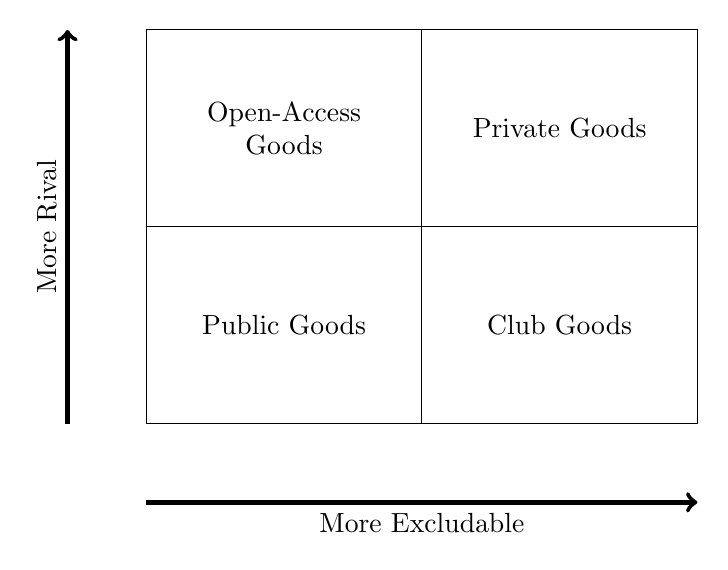
\begin{tikzpicture}[scale = 0.5]
		\draw (0,0) rectangle (7,5) node[pos=.5] {Public Goods};
		\draw (7,5) rectangle (14,10) node[pos=.5] {Private Goods};
		\draw (0,5) rectangle (7,10) node[pos=.5, text width = 2.7cm, align=center] {Open-Access Goods};
		\draw (7,0) rectangle (14,5) node[pos=.5] {Club Goods};
		\draw[ultra thick, ->] (0,-2) -- (14, -2) node[pos =.5, below]{More Excludable};
		\draw[ultra thick, ->] (-2, 0) -- (-2, 10) node[pos =.5, above, rotate=90]{More Rival};
	\end{tikzpicture}
	\vspace{1em}
	\fignote[1]{The goods matrix depicts the four main types of goods: private goods (excludable and rival), public goods (non-excludable and non-rival), open-access goods (non-excludable and rival), and club goods (excludable and non-rival). Although these are cannonically presented in four categories, the excludability and rivalry of goods is best thought of as taking place on a continuum.
	}
\end{figure}

A clean atmosphere is firmly a public good. There is no way to prevent people from benefiting from a healthy atmosphere with greenhouse gases at a level that supports climate stability, and one person's benefit does not infringe on another's. By the same virtue, greenhouse gas emissions are a public bad. No individual can exclude herself from climate change, and one person's climate damages do not prevent someone else from also experiencing those same damages. 

Defining a clean atmosphere as a public good provides a grounded explanation for why socially efficient greenhouse gas emissions abatement is unlikely to occur in the absence of public policy. All public goods struggle to find buyers. This lack of buyers is not necessarily because few people are willing and able to pay for the public good, but because these people do not have the proper incentives that would motivate them to actually buy into the public good. To see this, suppose there are two cities $A$ and $B$ on either side of a lake that is currently polluted and covered in algae blooms. Both cities benefit from the clean water in the lake through greater aesthetic appeal, higher property values, and increased ecotourism. As we have described it, clean water in the lake is a public good. Neither city can exclude the other from enjoying the clean water and one city's enjoyment of the clean water does not inhibit the other city from enjoying the clean water. 

\begin{figure}
	\caption{Market for a Public Good \label{mkt_public_good}}
	\centering
	\begin{tikzpicture}[scale=0.6]
		\draw[ultra thick, color1, domain=0:12] plot (\x, {4 - .25*\x}) node[right]{MB$_A$};
		\draw[ultra thick, color6, domain=0:12] plot(\x, {6 - .25*\x}) node[right]{MB$_B$};
		\draw[ultra thick, color3, domain=0:10] plot(\x, {\x}) node[right]{MC};
		\draw[ultra thick, color2, domain=0:12] plot (\x, {10 - .5*\x}) node[right]{MSB};
		\draw[thick, dashed] (3.2, 0) node[below]{$Q^A$} -- (3.2, 3.2) -- (0, 3.2) node[left]{$p^A$};
		\draw[thick, dashed] (4.8, 0) node[below]{$Q^B$} -- (4.8, 4.8) -- (0, 4.8) node[left]{$p^B$};
		\draw[thick, dashed] (6.667, 0) node[below]{$Q^S$} -- (6.667, 6.667) -- (0, 6.667) node[left]{$p^S$};
		\draw[ultra thick, <->] (0,10) node[left]{$p$} -- (0,0) -- (13,0) node[below]{$Q$ of Clean Water};
	\end{tikzpicture}
	\vspace{1em}
	\fignote[1]{Figure depicts a market for an emissions-intensive good, such as gasoline, based on Figure 5.4 in \cite{keohane2016markets}. In the figure, $p$ denotes the price of the good, $Q$ denotes the quantity of clean water, MC denotes the marginal cost of clean water, MB$_A$ denotes the marginal benefit of clean water to city $A$, MB$_B$ denotes the marginal benefit of clean water to city $B$, MSB denotes the marginal social benefit which is the sum of MB$_A$ and MB$_B$. The figure demonstrates that even in the smallest of public good provision situations, the equilibrium production of the public good be less than the socially efficient.}
\end{figure}

Figure \ref{mkt_public_good} displays the market for clean water. In this figure, MB$_A$ and MB$_B$ represent city $A$'s and city $B$'s marginal benefit from clean water respectively. The marginal social benefit (MSB) is the sum of the marginal benefits of each city for clean water. Both cities face the same marginal cost curve (MC) to improve the water quality. The socially optimal (i.e., total welfare maximizing) quantity of clean water is where the marginal cost of cleaning the water is equal to the marginal social benefit of the clean water, $Q^S$. However, the cities do not have the incentives that would drive them to this level of clean water. Individually, each city only will clean water to the point where the city's marginal benefit is equal to the marginal cost---$Q^A$ for city $A$ and $Q^B$ for city $B$. 

The provision of a public good leads to what is commonly known as the free-rider problem. Note that MB$_A$ is less than MB$_B$ indicating that city $B$ will always value improvements in water quality more than city $A$. In equilibrium, city $A$ will recognize this and choose not to produce any clean water. To see why start by supposing that city $A$ produces its privately optimal quantity of clean water $Q^A$. At $Q^A$, city $B$'s marginal benefit is still greater than its marginal cost, so it will also produce clean water in up until its marginal benefit is equal to the marginal cost. That is, city $B$ will produce $Q^B - Q^A$ of clean water such that the total quantity of clean water in between the two cities is $Q^B$. Now suppose instead that city $A$ chooses to produce nothing. Again city $B$ will choose to produce clean water up until its marginal benefit is equal to the marginal cost, such that the market quantity is $Q^B$. In both of these scenarios, the final market quantity is $Q^B$, but in the first scenario city $A$ also had to pay for the provision of the public good while in the second scenario city $A$ did not. Because city $A$ could end up with just as much of the public good when it does not contribute to its provision, then in equilibrium, city $A$ will not contribute or will ``free ride'' off of city $B$. Left to their own private incentives, city $A$ and city $B$ together will only ever produce $Q^B$, less than the socially optimal quantity of clean water, $Q^S$. 

The example with just two agents demonstrates that left only to their own private incentives, agents will typically provide less of a public good than is socially optimal. This result is apparent when there are even just two agents, but it is not difficult to imagine what this looks like when there are many agents. Even if there were 1000 agents, this model would still predict that only the one agent with the greatest marginal benefit would contribute to the provision of the public good---a quantity surely far less than the socially optimal quantity. 

% City $B$ cannot free ride off of city $A$ because its marginal benefit is greater for every quantity of clean water. Because of this city $A$ can choose not to contribute at all to the public good, understanding that city $B$ values clean water more and will clean any water that city $A$ would otherwise be willing to clean itself. In the end, the two cities will only end up producing $Q_B$ of clean water, less than the socially optimal amount. 

With this discussion of public good provision in mind, consider again whether or not it is possible to prevent future climate change in the absence of public policy. A clean atmosphere is a public good and as such, economists would expect that agents left to their own private incentives will provide far less of the public good than socially optimal. Left to our individual incentives, the atmospheric concentration of greenhouse gases will stabilize at a level far greater than and at a time far later than socially optimal. Absent of public policy, the world would need to find other ways to coordinate and resolve the externality.

Economists have explored alternatives to public policy that allow agents to resolve externalities and coordinate with each other without formal government intervention. In some instances, economic actors can in theory internalize the externality through bargaining, a result known as the Coase theorem \citep{coase1960problem}. Consider a classic example of the Coase theorem in practice from \cite{keohane2016markets}. In the late 1980s a bottled water company in France named Vittel had been incurring greater water purification costs as farmers in the neighboring communities had started using more potent fertilizers and spraying more chemicals on their farmland. These farming practices provide another example of an externality: the farmers used chemicals on their land that spilled over into the water supply, creating a cost that was not incurred by any of the farmers but by the bottled water company. To resolve this, the bottled water company paid farmers upstream to adopt less intensive farming practices. This benefits the bottled water company so long as payments to the farmers are less than the cost of the additional water purification. It also benefits the farmers provided that the payments they receive from the bottled water company are greater than the additional profit they would make from using the chemical treatments. Through this system, all parties gained (what economists might call a pareto improvement) and the externality was successfully internalized. 

Unfortunately, the Coase theorem has no bite in the context of climate change. For the Coase theorem to hold even theoretically, there must be enforceable property rights and transaction costs must be negligible. These transaction costs are often substantial, especially when dealing with many different actors and assessing compliance is difficult. Because climate change involves quite literally every person on the planet (and many more people not yet born), it suffices to say that the Coase theorem does not offer a legitimate approach to prevent future climate change. Further, Coasean bargaining may have potentially troubling distributional consequences. Recall that in the example the perpetrators of environmental damage (the farmers) received payments from those most harmed by this damage (the bottled water company). In the context of climate change, this would be the equivalent of suggesting that many of the low-income people of the world should pay the highest-income people of the world to reduce their greenhouse gas emissions. Clearly the Coase theorem does not provide a realistic or even preferably strategy to mitigate climate damages. 

Another alternative to public policy follows the work of \cite{ostrom1990governing}. Elinor Ostrom famously detailed instances from around the world where non-government institutions were able to successfully sustain natural resources including grazing land, forests, and groundwater aquifers in her landmark book \textit{Governing the Commons}. In each of these cases, individuals and firms organized themselves together to resolve ``collective action problems" and protect natural resources. 

Could similar approaches like those Ostrom studies succeed in creating climate action at the necessary scale? It is highly unlikely. Ostrom focuses on open-access resources, where a healthy atmosphere is firmly a public good (alternatively, greenhouse gas emissions are a public bad). Much of her analysis is based on the rivalry of the resources and consequently does not translate well for reducing emissions. More importantly, some of the key features that allow these self-governance approaches to succeed are not met in the context of climate change. The systems Ostrom studies are primarily local and rely on mutual-monitoring and enforcement. Given the global nature of climate change and the invisibility of greenhouse gas emissions, it would be a tremendous leap to say that climate action is achievable through self-governance and collective action alone. 

Putting these pieces together, individual firms and consumers will produce far too many greenhouse gas emissions as the costs they face do not reflect the greater societal costs of their actions. These same firms and consumers will fail to produce a cleaner atmosphere, a necessary public good, because they cannot exclude others from enjoying the benefit of a clean atmosphere. Without this ability to exclude, many of those willing to produce a cleaner atmosphere will not do so because they are able to ``free ride'' off of other agents who are willing to pay for a cleaner atmosphere. Individuals left to their own incentives will not be able to reduce their greenhouse gas emissions. Alternatives to public policy, like the Coasean bargaining and collective action, are not able to scale at the level necessary to create global emissions reductions. The only option that remains is public policy. 

Even with domestic climate policy, this of course still leaves room for free riding at the global level. However, with a public policy focus in mind, the relevant actors are no longer individuals but entire nations. This change drops the number of relevant actors from billions to just dozens, making the prospect of cooperation far more likely. Currently, international cooperation has been mostly limited to voluntary climate pledges like the defunct Kyoto Protocol or the Paris Climate Agreement, where the compliance and enforcement of commitments is ambiguous at best. There are however other, more enforceable options at the international level to promote cooperation and prevent nations from shirking on their climate obligations. The most prominent of these approaches is likely the idea of a ``climate club,'' popularized by \cite{nordhaus2015climate}. A climate club is a group of nations that imposes trade penalties on other nations that do not fulfil their climate obligations, providing some incentive for nations to create policy that reduces their emissions profiles. Climate clubs are already beginning to emerge informally through the implementation of the European Union's recently revised Carbon Border Adjustment Mechanism (CBAM), which levies trade restrictions in Europe against imports from nations with relatively emissions intensive production processes. Section 2.5 contains a more thorough discussion of Border Carbon Adjustments (BCAs).





% The market failure that leads to climate change is less of a market failure and much more of a market omission. The omission of the market for a clean atmosphere creates ragged, incomplete edges in adjacent emissions intensive markets. 





% For the sake of simplicity, assume that all technology needed to attain net-zero emissions and stablize the concentration of greenhouse gases in the atmosphere was commercially available. Even if this was the case, 

% Overall, when a good is non-excludable, it is difficult to create an incentive structure that motivates individuals who value the public good to contribute to its provision. The field of mechanism design studies these incentive structures, as called ``mechanisms,''  with the intent of motivating individuals to reveal their private value for a public good and contribute this value to its provision. \footnote{See Chapter 7 of \cite{fudenberg1991game} for the authoritative treatment on the application of mechanism design to public good provision problems.} These mechanisms are mathematically complex, and ultimately always rely on a social planner to implement and enforce

% Economists often use the classic prisoners' dilemma game to model a public good contribution game. 

% All agents have a strictly dominant strategy to not contribute towards the public good, provided that they would prefer to not contribute to the public good and not receive it than finance the public good individually. A coal-burning power plant wants to prevent climate change damages, but preventing these damages will require sweeping action from around the world. It could not successfully mitigate climate change damages by itself, and even if it could, the costs involved would far exceed its benefits. If other actors choose to take aggressive action on climate change, then making serious abatement efforts costs the coal plant but provides no benefit. In either case, the plant is better off doing nothing. The universal, non-excludable nature of the benefits of climate change mitigation fails to create the proper incentives for individual actors to take action.\footnote{The rivalry of goods tends to be less important than their excludability in environmental contexts. \cite{hardin1968tragedy} famously considered the example of an English pasture to show that agents will overexploit non-excludable but rival goods, leading to the collapse of the natural system, provided the agents have no institutions that can enforce cooperation. For this reason, the excludability is the primary concern in the environmental and climate settings.}

% Absent any additional incentive, individual agents will fail to implement the necessary changes. 

%This implies that in certain circumstances, private agents can resolve externalities without public policy. 

% In summary, economic theory posits that agents will produce excessive greenhouse gas emissions because they do not face the full social consequences of their economic activities. A safe and stable atmosphere is public good, and consequently, private agents do not have an incentive to abate their emissions. Without policy intervention, the resulting equilibrium outcome will 

% Although non-policy options exist to internalize the externality (e.g., Coasen strategies) or cooperate towards more socially desirable outcomes (e.g., collective action strategies), the number of relevant parties means these are not serious alternatives to public policy. 

% The next section briefly address the suite of policy available 

\subsection{The Structure \& Scope of Environmental Policy \label{2.3}}

So far, this chapter has motivated the use of public policy to manage climate change damages by using economic theory to discuss why the alternatives to public policy will not be able to prevent future climate change. While this is an important step, this ultimately falls short of demonstrating that public policy has the potential to reduce greenhouse gas emissions. The goal of this section is to fill in this gap by providing an overview of common forms of environmental policies and briefly outlining how they reduce greenhouse gas emissions. Of course this short section cannot survey all available forms of climate policy, but it does provide enough context on the variety of policies available for the chapters that follow. Major themes from this discussion come from \cite{keohane2016markets}, and Figure \ref{policies} visualizes the scope of policies described. 

Perhaps the most famous treatment of the difficulty managing non-excludable goods---a category that includes most environmental goods---is ``The Tragedy of the Commons,'' by American ecologist Garrett Hardin.\footnote{The ``Tragedy of the Commons'' allegory did not first appear in \cite{hardin1968tragedy}, but the work of British writer William Forster Lloyd. \cite{lloyd1833two}  contains the first known use of the pasture allegory. It is also worth noting that in both Lloyd and Hardin's works, the allegory is used to make a broader argument about the unsustainability of population growth, whereas today it is generally used to discuss environmental degradation. The Malthusian arguments made in both works are easily refuted today as wealthy, industrialized nations have seen declining birth rates but sustained economic growth.} In his controversial essay, Hardin primarily discusses the trouble in managing this class of goods where in their common form they are non-excludable. On the management of significant natural landscapes like National Parks,  Hardin writes:
\begin{quote}
\singlespacing ``What shall we do? We have several options. We might sell them off as private property. We might keep them as public property, but allocate the right to enter them… These, I think, are all the reasonable possibilities.''
\end{quote}
In this passage, Hardin presents a dichotomy for allocating many environmental goods: privatization or nationalization. Both of these options are similar in that they rely on making a non-excludable good excludable by giving entities sole control over a portion (or the entirety) of the good, but different in how they determine the final allocation of the good. Privatization of a good uses market forces to allocate and manage the good, whereas nationalization of a good uses the state to allocate and manage the good. Although the empirical validity of Hardin's dichotomy is questionable,\footnote{Ironically, the goods that are least likely to be managed in the ways Hardin describes are the open-access goods he focuses on. In the first chapter of her book, \cite{ostrom1990governing} challenges this dichotomy and proceeds through the book detailing examples of well-managed open-access goods that are neither nationalized nor privatized. Ostrom won the Nobel prize in Economics for her work in 2009.} the bulk of modern environmental policy still parallels this basic dichotomy. Today most environmental policy can be classified as either a market-based policy or a command-and-control policy.

% In Garrett Hardin's classic paper ``The Tragedy of the Commons,"  he proposes two approaches to managing open-access resources: privatization and nationalization. The key in both cases is consolidating agents, who would otherwise experience the consequences of each others' actions but not their own, under one umbrella. When there is only one party in charge, there is no room to free ride.\footnote{It is worth noting that an $N$-player ``Tragedy of the Commons'' game is functionally identical to an $N$-player Cournot game. This highlights how the market behavior of a monopoly ($N =1$), under-producing and over-pricing a good, can actually become socially desirable in the case of environmentally damaging goods, which are usually over-produced and under-priced. Privatization and nationalization of the commons both amount to granting a monopoly on a good.} The difference is of course the motivation of these agents. Under privatization, the management of the commons is conducted through market forces, while under nationalization, the management of the commons is conducted through government supervision. 

% Today, many environmental policies still fall into a dichotomy that parallels the dichotomy Hardin discussed: market-based policies and command-and-control policies.\footnote{Ironically, perhaps the goods that are least likely to be managed in the ways Hardin describes are the open-access goods he focuses on. In the first chapter of her book, \cite{ostrom1990governing} challenges this dichotomy and proceeds through the book detailing examples of well-managed open-access goods that are neither nationalized nor privatized.} Market-based policies manage the environment through market forces, while command-and-control policies manage the environment through prescriptive government directives. This section proceeds by unpacking these groups of policies identifying common forms for these policies to take place it, and reflecting on the strengths and weaknesses of these policies. 

Command-and-control policies are what we would typically think of as environmental regulation. In the context of a non-excludable environmental good, a command-and-control policy is any policy where the state determines the allocation of the good. More commonly, a command-and-control policy is any policy where government creates specific prescriptions to firms and possibly consumers. For this reason, command-and-control policy is also often called prescriptive policy. Command-and-control policies often involve some combination of prohibition/permission and standard setting. 

Prohibition policies prevent actors from taking certain actions, like purchasing a piece of land (i.e., giving ownership of the land to the state) or disposing of a hazardous chemical in certain locations. These typically appear in the management of public lands, like National Parks, Wildlife Refuges, and Forests. Often alongside prohibition is permission, where government may for instance lease National Forests to the logging industry or grant rights to a firm to drill for oil on state-owned land. In a loose sense, we might also classify any policy enforcement as a part of this category. Regulators may prohibit certain activities with prescribed punishments for violators. 

Another approach to regulating and protecting the environment is through standard setting. Standards generally come as either \emph{technology standards} or \emph{performance standards}. Technology standards require firms to use specific technologies. Many coal-burning power plants must install smokestack scrubbers to prevent damaging chemicals from entering the lower atmosphere. Alternatively, performance standards do not specify specific technologies, but set bounds on the rate or total magnitude of an environmental impact. This could involve setting an emissions cap on an individual firm or car fuel economy standards, which indirectly govern the rate of carbon dioxide emissions per mile. Technology standards provide the characteristic inflexibility of a command-and-control policy, but performance standards can provide somewhat more flexibility. For instance, the Clean Air Act establishes air quality standards for entire regions but leaves it up to local jurisdictions how to meet these air quality standards. This could very well involve the use of market-based strategies to determine air quality improvements that will allow an area to meet the performance standard.


Market-based policies are the foil to command-and-control policies. Rather than using the state to allocate environmental goods, market-based policies use markets to allocate these goods. Recall from the previous section that an important reason environmental goods like a clean atmosphere are often underprovided is that the markets for these goods are often ``incomplete'' in the sense that there are costs or benefits that do not appear in the natural state of the market. For instance, emissions damages do not appear in the market for gasoline. Alternatively, the market for a public good is incomplete because only the agent with the greatest marginal benefit will participate, leaving the benefits of the many other agents that benefit from the provision of the good out of the market. The core idea of market-based policies is to overcome these market failures by completing the market. \cite{keohane2016markets} make this point clear, writing ``the problem is not that markets are so pervasive but that they are not pervasive \emph{enough}---that is, they are incomplete." 

This claim that public policy can resolve a market failure by creating more markets should not be taken at face value. Market-based policy is entirely ironic. In a scenario where markets have failed to provide the socially optimal levels of an environmental good, market-based policy suggests that the solution is to create new markets. Are economists naive to suspect that the same free-market principles that cause environmental issues can actually resolve them? The section that follows considers these policies in greater detail, backing up this bold presumption first with theory and then with empirical evidence on market-based climate policy. 

Policymakers primarily conduct market-based policy by setting either a price or a quantity of an environmental good, the two components of a market. Price instruments are the traditional Pigouvian solution. When there is a market failure due to some externalitiy, we can internalize the externality by taxing or subsidizing a good so individual incentives will align with social incentives. Carbon taxes are a clear example of this strategy. There are costs of carbon dioxide emissions that do not appear in the prices of goods and activities that rely on these emissions. Consider the example of a driver purchasing gasoline from section \ref{2.2}. In this example, a gallon of gasoline causes \$1.64 in climate damages. A Pigouvian-style carbon tax of \$1.64 would charge an additional \$1.64 for every gallon of gasoline (likely on the consumption of gasoline), which will internalize the externality---forcing the financial incentives of agents in the market to align with the underlying social incentives. Unlike common command-and-control policies, a carbon tax is flexible in the sense that agents can choose their level of abatement. Emissions will come at a cost, but with an economy-wide carbon tax, consumers could choose whether their emissions abatement comes through reducing electricity consumption, reducing gasoline consumption, or any other way someone might reduce their emissions. Price instruments often work in the other direction as well, incentivizing an activity of which there is currently too little. For instance, energy-efficient durable goods are often subsidized as a strategy to both reduce energy use and emissions. Similarly, renewable energy subsidies provide tax rebates for the installation of renewable capacity with the goal of overcoming investment inefficiencies and emissions reductions. 

Alternatively, policymakers might also use quantity-based instruments to create financial incentives. The typical example here is a cap-and-trade program, where policymakers require certain actors to own emissions permits or emissions allowances for every tonne of their greenhouse gas emissions. In the standard presentation of a cap-and-trade program (also widely known as an emissions trading program), policymakers create a fixed quantity of these permits with the option to sell these permits to regulated firms. If firms were only allowed to keep these emissions allowances, then this would be equivalent to a performance standard. The differentiating element here is the tradeable nature of these allowances. Under a cap-and-trade program, firms can buy and sell these emissions allowances from each other. This creates a market for allowances, which puts a price on emissions. Just like a carbon tax, the price of an emissions allowance creates a financial incentive for emissions abatement. Other programs outside of the reduction of greenhouse gas emissions make use of quantity-based instruments. For instance, Wetland Mitigation Banking in the US fixes a quantity of land for wetland conservation. Firms and farmers that wish to develop on existing wetland must offset this development by building or conserving a tract of wetland equivalent to the wetland they displace through development. 

There are of course policies that are best understood as a combination of command-and-control and market-based policies. 
For instance, information tools can use a combination of both command-and-control and market-based policies. A mandatory eco-labeling program might require firms to display the carbon footprint of a good they sell. This a specific reporting requirement without a direct financial incentive attached to the policy. Still, consumers, seeing this information might change what and how many products they purchase. This creates secondary financial incentives for firms, similar to a market-based policy. Sometimes these programs are not mandatory, and firms  voluntary participate in labeling due to some financial incentive. Other times, there is no financial incentive for information disclosure, but regulators require disclosure regardless. This is the case in program's like the EPA's Greenhouse Gas Emissions Reporting Program. This program requires facilities that potentially have high emissions to collect data and report on their greenhouse gas emissions.

As important as it is to understand the range of policies available, ultimately, policymakers need to know what the most effective policy is. Unsurprisingly, the answer to this question depends on how ``effectiveness'' is measured. Economists often focus on welfare maximization (equivalently, cost minimization) as a policy objective. In the context of greenhouse gas emissions, the best policy would be able to abate $x$ tonnes of emissions at the lowest cost. For this reason, economists tend to favor market-based over command-and-control policy. Market-based instruments, like a carbon tax or a cap-and-trade program, are understood to minimize the cost of emissions abatement where command-and-control policies do not. This minimization is due to the flexibility of markets to allocate abatement to those agents that can abate their emissions at the lowest cost. This does not matter if all agents have the same marginal cost of abatement, but in the realistic case where agents have heterogeneous abatement cost curves, command-and-control policies will not have the information needed to allocate abatement in a cost-minimizing fashion. 

A second important advantage of market-based policies is that these programs create incentives for firms to invest in research and development of new technologies with positive environmental impacts. Consider how a best-available technology (BAT) standard affects research and development incentives. Under a BAT standard, firms are required to adopt the best commercially-available technology for pollution reductions. In this case, firms have an incentive to collude and collectively invest nothing into new technologies that would lead to better abatement than what is currently available. Firms will have a mutual understanding that any improvements in abatement technology will mean all firms must undertake a costly process to adopt the new technology---potentially leading these firms to even suppress better technologies they find. Under a market-based policy though, firms would have a strong incentive to invest in abatement technology research. If a firm can learn how to lower its own abatement costs, then it will be able to reduce its own burden from the policy and gain a competitive advantage over other firms in the industry.

Despite the merits of market-based approaches to public policy commonly touted by economists, price and quantity instruments are no panacea. One significant concern in many areas of environmental policy is enforcement. Natural resources are often incredibly large and it is difficult to monitor individual behaviors that relate to these resources. The earlier discussion on the cost-minimizing nature of these market-based approaches excludes any consideration of enforcement costs, and when we include these enforcement costs, this result does not necessarily hold. 

As an example, suppose a policymaker had the objective of reducing bycatch on commercial fishing vessels at the lowest cost. Bycatch is when fishers unintentionally catch and kill sealife like dolphins or sea turtles instead of the fish they intended to catch. There are ways fishers can mitigate bycatch, like modifying nets with visual or auditory stimuli that the intended species will not respond to but the other species will avoid \citep[for example, see][]{bielli2020illuminating}. Consider a market-based strategy to reduce bycatch, like taxing fishers for the non-targeted sea life that they catch and kill. If fishers followed this rule, the tax would be enough for many of them to adopt the technologies that would reduce bycatch. This would minimize the total costs incurred by fishers. Fishers who face high costs from reducing bycatch will barely reduce their bycatch as they would rather pay the tax. Fishers who face low costs from reducing bycatch will greatly reduce their bycatch as they would rather adopt new technologies than pay a tax. Of course, this assumes that there is perfect compliance and enforcement is costless. What kind of costs would be involved in enforcing a tax like this? Monitoring and taxing the bycatch of every commercial fisher in an area would be tremendously difficult and expensive. We do not have the technology to monitor every animal caught in every commercial fishing net. Even if there was a monitoring official on every large commercial fishing vessel, there would be strong incentives for collusion. 

In situations where enforcement is incredibly costly, it may be more cost-effective to take a command-and-control approach that prescribes uniform policies across actors. In this example, it would be much less expensive to require that commercial fishers use bycatch-reducing nets. Policymakers could incorporate this into existing procedures for commercial fishing licensing and even prevent the production and sale of more harmful nets. This policy would not be cost-minimizing for the fishers, but if the difference in enforcement costs was large enough, it may be more cost-minimizing to society as a whole. A technology standard, a command-and-control approach, seems more appropriate in this case.

More important to the remainder of the paper are the distributional concerns with market-based policy instruments. In the context of environmental goods and bads, there are two primary distributional concerns with market-based policy. The first concern is that because many forms of pollution violate the uniform-mixing assumption, market-based policies may not actually be cost-minimizing. The uniform mixing assumption holds that pollutants will mix such that the concentration of the pollutant is homogenous throughout a substance. In practice, the uniform mixing of pollutants means that the location of pollution does not matter. A unit of pollution at location A will have the same impact as a unit of pollution at location B, as this pollution will distribute itself across all locations regardless of where it comes from. The uniform mixing assumption holds in the case of greenhouse gas emissions; one tonne of CO$_2$ in Los Angeles causes just as much damage as one tonne of CO$_2$ in the middle of Iowa. The uniform mixing assumption does not hold in the case of criteria air pollutants; one pound of particulate matter (PM) in Los Angeles causes more damage than one pound of PM in the middle of Iowa. This is significant because criteria air pollutants will have consequences that vary based on their location, but the price they face from a market-based instrument will be homogenous. When this is the case, the major appeal of market-based policies no longer holds; quantity and price instruments are no longer necessarily cost minimizing. In fact, if marginal abatement costs are similar across firms and government can estimate the difference in their marginal impacts, then a command-and-control policy could very well lead to a greater total welfare than a market-based policy.

The second primary distributional concern with market-based policy is not truly a concern with the policy itself, but the goal of this policy. Even if market-based policy results in the welfare-maximizing allocation of an environmental good or bad, this allocation is not necessarily made with equity in mind. Later chapters focus extensively on this criticism, so consider a motivating example. Suppose a state is interested in reducing PM  pollution from fossil fuel electric power generators at the lowest cost. With this objective in mind, economic theory would suggest that a cap-and-trade program on PM emissions may work well. Now suppose instead that the state is interested in reducing PM pollution while also eliminating the disparity in PM pollution between neighborhood A and neighborhood B. Market-based policy is not well-suited for this task. It is entirely possible that a cap-and-trade program on PM pollution could force the closure of high-abatement cost generators in neighborhood A, shifting generation and PM pollution to lower-cost abatement generators in neighborhood B. In doing so, this market-based policy could actually increase the disparities in PM pollution between neighborhoods. It could just as well do nothing to change disparities in PM pollution, or even lower disparities in PM pollution. The upshot of this is that market-based policies use markets to allocate environmental goods and bads, and because markets do not allocate goods and services with distributional concerns in mind, these policies are poorly suited to situations where eliminating disparities is a primary objective. 

This section has focused on describing a range of environmental and climate policies and their relative merits. Market-based policies use markets to allocate environmental goods, whereas command-and-control use the state to allocate environmental goods. While traditionally economists favor market-based policies due to their cost-minimizing nature, these policies are not universally superior to command-and-control policies. Importantly, these policies cannot guarantee a ``fair'' distribution of environmental goods, a point that returns later in the text.



\subsection{Environmental Markets: Carbon Taxes \& Cap-and-Trade}

Market-based policies to reduce greenhouse gas emissions, like carbon taxes and cap-and-trade programs, are the economics profession's instrument of choice to prevent future climate change. The goal of this section is to address these policies in detail, unpacking how carbon pricing functions both in theory and in practice. 

\subsubsection{The Theory of Carbon Pricing}

Carbon pricing is a term used for market-based policies that ``put a price'' on greenhouse gas emissions, like a carbon tax or a cap-and-trade program for greenhouse gas emissions. Recall that market-based policies function by creating a complete market out of an incomplete market. In the context of climate change, this incomplete market is the market for emissions abatement (the economic good) or equivalently the market for emissions (the economic bad). Figure \ref{c_pricing} displays these markets. 

First consider the market for abatement, shown in Figure \ref{abatement1}. The supply of emissions abatement is equivalent to the marginal abatement costs (MAC). Towards the left of the MAC curve are the low hanging fruit of abatement options.\footnote{Some empirical estimates of this curve suggest that this far portion of the MAC may actually be negative. That is, initial emissions abatement is achievable at a negative cost, as firms and individuals can often save money through energy-efficiency improvements. This is related to the energy-efficiency gap \citep[see][]{allcott2012there, gerarden2017assessing}.} As more abatement occurs, the technologies involved in abatement become more costly, and many of these require new research investments into technologies that are not yet available. Although there are private costs involved in emissions abatement, there are also social gains. These gains are equivalent to avoided climate change damages. Marginal damages increase with the quantity of emissions; the more emissions are already in the atmosphere, the greater the impact of an extra tonne of CO$_2$. For this reason, the marginal benefits of abatement are decreasing. The first tonne of CO$_2$e abated is responsible for the largest reduction in climate change damages, and any subsequent abatement is less effective at reducing damages. Abatement is a public good though, so despite the social benefits, no private agents are willing to pay for abatement. 

Market-based policies attempt to resolve this issue by using government to act as a ``demander" of abatement. In the conventional framing, it is impractical for policymakers to set a full demand curve for abatement, so instead policymakers can set a simple demand curve that will still bring the market to its true equilibrium. Namely, a policymaker can set a horizontal demand curve for abatement at $p^*$ or a vertical demand curve for abatement at $A^*$. These two options are identical in simple models of abatement as both lead to the socially optimal level of abatement. 

\begin{figure}
\caption{Creating a Market for a Public Good (or Bad)\label{c_pricing}}
\centering
\subcaptionbox{The Market for Abatement \label{abatement1}}{
\begin{tikzpicture}[scale=0.37]
	\draw[very thick, <->] (0,10) node[left]{$p$} -- (0,0) -- (13,0); 	
	\draw[very thick, color2, domain=0:12] plot(\x, {.6*\x + 1}) node[right]{\footnotesize S = MAC};
	\draw[very thick, color1, domain=0:12] plot(\x, {-.4*\x + 9}) node[right]{\footnotesize D = MB}; 
	\draw[very thick, lightgray] (8,0) node[below, black]{$A^*$} -- (8,10);
	\draw[very thick, lightgray] (0,5.8) node[left, black]{$p^*$} -- (13,5.8);
	\draw[very thick] (11, 0) node[below]{$A_\text{Max}$} -- (11, 10);  
	\node[below] at (6.5, -3) {Abatement ($A$)};
	\draw (9.5, -2) node{$\underbrace{~~~~~~~~~~~}_{E^*}$};
\end{tikzpicture}
}
\hspace{.01cm}
\subcaptionbox{The Market for Emissions \label{emissions1}}{
\begin{tikzpicture}[scale=0.37]
	\draw[very thick, <->] (0,10) node[left]{$p$} -- (0,0) -- (13,0);	
	\draw[very thick, color2, domain=0:12] plot(\x, {7.6 - .6*\x}) node[above right]{\footnotesize D = MB};
	\draw[very thick, color1, domain=0:12] plot(\x, {4.6 + .4*\x}) node[right]{\footnotesize S = MSC};
	\draw[very thick] (11, 0) node[below]{$E_\text{Current}$} -- (11, 10);
	\draw[very thick, lightgray] (3,0) node[below, black]{$E^*$} -- (3,10);
	\draw[very thick, lightgray] (0,5.8) node[left, black]{$p^*$} -- (13,5.8);	
	\node[below] at (6.5, -3) {CO$_2$e Emissions ($E$)};
	\draw (7, -2) node{$\underbrace{~~~~~~~~~~~~~~~~~~~~~~~~~~~~~~~}_{A^*}$};
\end{tikzpicture}
}
\vspace*{1em}
\fignote[1]{
	Figure presents two equivalent markets: (a) the market for abatement, and (b) the market for emissions. In the market for abatement D = MB is the demand for abatement or the marginal benefit of abatement, where the marginal benefit of abatement is equal to the marginal value of avoided damages; S = MAC is the supply of abatement or the marginal abatement cost; $A_\text{Max}$ is the maximum level of abatement, equal to the current level of emissions; $A^*$ is the equilibrium value of abatement; and $p^*$ is the price of abatement. In the market for emissions D = MB is the demand for emissions or the marginal benefit of emissions, where the marginal benefit of emissions is equal to the marginal value of avoided abatement; S = MSC is the supply of emissions or the marginal social cost of emissions; $E_\text{Current}$ is the current level of emissions; $E^*$ is the equilibrium level of emissions; and $p^*$ is the equilibrium price of emissions. The market for abatement and the market for emissions correspond such that the price of abatement and the price of emissions are the same, $A_\text{Max} - A^* = E^*$, and $E_\text{Current} - E^* = A^*$. Horizontal gray lines illustrate a hypothetical carbon tax and vertical gray lines illustration a hypothetical emissions cap.
}
\end{figure}

The previous example framed market-based instruments from the perspective of creating a market for emissions abatement, an approach that highlights how government intervention can work to establish a market for a public good. Although this framing is important and one that is often more convenient, the interpretation and public policy implications can seem counterintuitive. With government on the demand side, this would imply a policy where government pays polluters to abate, either promising a fixed rebate on each tonne of emissions abated or by purchasing abatement until it reaches $A^*$. In this system, polluters would earn more revenue through abatement. Major climate policy proposals do not include such massive payoffs to polluters, and rightly so; in the long run these economic profits would attract more firms to enter high-polluting industries and diminish the efficacy of the policy. There may also be additional social costs if the government reduces other expenditures or raises taxes in order to finance these payouts. 

The familiar policies focus on the inverse of the abatement market, the market for emissions. This market appears in Figure \ref{emissions1}. In this market, the government does not intervene to demand a public good, but to establish rights for and supply a public bad. The polluters derive their demand for emissions from their MAC curves, representing the most polluters will be willing to pay for the right to send CO$_2$e emissions into the atmosphere rather than abate. The supply curve in this market is the marginal damage of emissions. This framing comes with a clearer interpretation. Here, policymakers impose a carbon tax---a charge of $p^*$ on each tonne of CO$_2$e emissions. In equilibrium, this tax will lead to total emissions $E^*$. A cap-and-trade program instead sets a vertical supply curve of emissions allowances that give polluters the right to emit one tonne of CO$_2$e, at $E^*$. A key feature of these allowances is that they are tradeable between polluters. Although it is not necessary for government to sell or auction off emissions allowances, if government did, their equilibrium price would be $p^*$. 

Figure \ref{c_pricing} illustrates that the market for abatement and the market for emissions correspond. The difference between the maximum level of abatement and the equilibrium level of abatement is the equilibrium emissions, and the difference between the current level of emissions and the equilibrium level of emissions is the equilibrium abatement. The market price for emissions is the same as the market price for abatement. Framing market-based policy through the market for emissions has a more convenient interpretation relative to standard policy. However, because the prices and quantities are identical in both markets, economists often choose to frame market-based polices through the market for abatement rather than the market for emissions. This approach can be clearer when considering the cost-minimizing nature of market-based instruments.

The market for emissions also illustrates the equivalence of carbon pricing and a cap-and-trade program \emph{when the market is in equilibrium}. Every price on emissions corresponds with a single emissions cap, and every emissions cap corresponds with a single price on emissions. In this sense, a carbon tax and a cap-and-trade program are equivalent. Of course over time the marginal benefits curve will shift, and when this happens, the original supply curve set by the policy will no longer maximize welfare in the market for emissions.\footnote{The marginal social cost curve will also shift overtime, but will do so in more predictable ways.} When this occurs, then a carbon price and cap-and-trade program are no longer equivalent. In simplistic models of an emissions market like in Figure \ref{emissions1}, the elasticity of the emissions demand curve is useful for determining whether a carbon tax or an emissions cap is preferable. If the emissions demand curve is relatively elastic, then a carbon tax will make the market for emissions less volatile. If instead the emissions demand curve is relatively inelastic, then an emissions cap will make the market for emissions less volatile.

\begin{figure}
\caption{Distribution of Allowances with Carbon Pricing\label{dist_allowance}}
\centering
\begin{tikzpicture}[scale=0.6]
	\fill[lightgray!50!, domain = 0:7, variable = \x] (0,0) -- plot(\x, {.09*\x^2}) -- (7,0) -- cycle;
	\fill[lightgray!50!, domain = 7:10, variable = \x] (7,0) -- plot(\x, {.1*(12-\x)^2 + 1.91}) -- (10,0) -- cycle;
	\draw (0,0) rectangle (10,8.33);
	\draw (0,0) node[below]{0} -- (10,0) node[below]{100} -- (10,8.33) node[above]{0} -- (0,8.33) node[above]{100} -- (0,0);
	\draw[very thick, ->] (10, 9.33) -- (0, 9.33) node[pos=.5, above]{Polluter 2's Abatement (tonnes)};
	\draw[very thick, ->] (0, -1) -- (10, -1) node[pos=.5, below]{Polluter 1's Abatement (tonnes)};
	\draw[very thick, color2, domain=0:9.603] plot(\x, {.09*\x^2});
	\draw[very thick, color1, domain=3.988:10] plot(\x, {.1*(12-\x)^2 + 1.91}); 
	\draw[thick, dashed] (0,4.41) node[left]{\$50} -- (7,4.41);
	\draw[thick, dashed] (7,8.33) node[above]{30} -- (7,0) node[below]{70};
	\draw[thick, dashed] (5,8.33) node[above]{50} -- (5,0) node[below]{50};
	\node[rotate=90, above] at (-1, 4.155) {Price (\$)};
	\node[color2] at (9, 5.5) {MAC$_1$};
	\node[color1] at (9, 1.5) {MAC$_2$};
	% \draw[lightgray, thick] (5,0) node[below, black]{50} -- (5,8.33) node[above, black]{50};
\end{tikzpicture}
\fignote[1]{The figure visualizes the abatement market for Polluter 1 and Polluter 2. Polluter 1's abatement increases along the bottom horizontal axis, and Polluter 2's abatement decreases along the top horizontal axis. This arrangement means that at any point along the horizontal axis, the total abatement between the two polluters will be 100 tonnes. MAC$_1$ and MAC$_2$ represent the marginal abatement cost curves of Polluters 1 and 2 respectively.The shaded areas under the marginal abatement cost curves represent the total cost of abatement.}
\end{figure}

\begin{figure}[!htbp]
	\caption{Distribution of Allowances with Command-and-Control Policy\label{allowance_cost}}
	\centering
	\begin{tikzpicture}[scale=0.6]
		\fill[lightgray!50!, domain = 0:5, variable = \x] (0,0) -- plot(\x, {.09*\x^2}) -- (5,0) -- cycle;
		\fill[lightgray!50!, domain = 5:10, variable = \x] (5,0) -- plot(\x, {.1*(12-\x)^2 + 1.91}) -- (10,0) -- cycle;
		\fill[color3!30!, domain=5:7, variable = \x] (5,4.3) -- plot(\x, {.1*(12-\x)^2 + 1.91}) -- (7,4.41) -- cycle;
		\fill[color3!30!, domain=5:7, variable = \x] (5,4.5) -- plot(\x, {.09*\x^2}) -- (7,4.41) -- cycle;
		\draw (0,0) rectangle (10,8.33);
		\draw (0,0) node[below]{0} -- (10,0) node[below]{100} -- (10,8.33) node[above]{0} -- (0,8.33) node[above]{100} -- (0,0);
		\draw[very thick, ->] (10, 9.33) -- (0, 9.33) node[pos=.5, above]{Polluter 2's Abatement (tonnes)};
		\draw[very thick, ->] (0, -1) -- (10, -1) node[pos=.5, below]{Polluter 1's Abatement (tonnes)};
		\draw[very thick, color2, domain=0:9.603] plot(\x, {.09*\x^2});
		\draw[very thick, color1, domain=3.988:10] plot(\x, {.1*(12-\x)^2 + 1.91}); 
		\draw[thick, dashed] (0,6.81) node[left]{\$68} -- (5,6.81);
		\draw[thick, dashed] (0,2.25) node[left]{\$23} -- (5,2.25);
		\draw[thick, dashed] (5,8.33) node[above]{50} -- (5,0) node[below]{50};
		\node[rotate=90, above] at (-1, 4.155) {Price (\$)};
		\node[color2] at (9, 5.5) {MAC$_1$};
		\node[color1] at (9, 1.5) {MAC$_2$};
		% \draw[lightgray, thick] (5,0) node[below, black]{50} -- (5,8.33) node[above, black]{50};
	\end{tikzpicture}
	\fignote[1]{The figure visualizes the abatement market for Polluter 1 and Polluter 2. Polluter 1's abatement increases along the bottom horizontal axis, and Polluter 2's abatement decreases along the top horizontal axis. This arrangement means that at any point along the horizontal axis, the total abatement between the two polluters will be 100 tonnes. MAC$_1$ and MAC$_2$ represent the marginal abatement cost curves of Polluters 1 and 2 respectively. The dotted vertical line represents a potential state allocation of abatement under a command-and-control policy. The shaded areas under the marginal abatement cost curves represent the total cost of abatement. Here, the yellow area represents the welfare loss incurred from the command-and-control policy.}
\end{figure}

Cap-and-trade programs come with the added complexity of determining how to initially distribute emissions allowances. It turns out that in our simple theoretical model of a cap-and-trade program with tradeable allowances, the initial distribution of allowances is irrelevant to whether or not the policy achieves the emissions reduction cost-effectively. Suppose that there are just two polluters in our system, Polluter 1 and Polluter 2, each of whom currently has 100 tonnes of emissions. The assumed benevolent policymaker wants to cut emissions in half by setting a cap of 100 tonnes of emissions between the two polluters. Polluter 1 and 2 have marginal cost of abatement curves depicted in Figure \ref{dist_allowance}. Consider two alternative scenarios: (1) the policymaker sells allowances to the polluters, and (2) the policymaker gifts 50 (tradeable) allowances to each polluter. 

If the policymaker sells allowances to the polluters, then both polluters will purchase allowances up until the price of an allowance equals the cost of an additional tonne of abatement. That is, each polluter will purchase the quantity of emissions allowances where the price of an allowance is equal to its marginal abatement cost. The demand for abatement is perfectly inelastic, so the equilibrium price will be where the sum of the quantities of abatement supplied by the polluters is 100 tonnes. Graphically, the total marginal abatement cost curve for the two polluters together is a horizontal summation of each individual marginal abatement cost curve. Figure \ref{dist_allowance} shows that at a price of \$50, the sum of Polluter 1 and 2's abatement is 100 tonnes, the desired level of abatement. Total abatement costs are equal to the area under each abatement curve from 0 to its level of abatement. 

Suppose instead each polluter begins with 50 allowances. If both have 50 allowances, Polluter 2 would have a far higher marginal cost of abatement than Polluter 1. Knowing this, Polluter 1 might sell some of its allowances to Polluter 2. Polluter 1 will sell its allowances as long as the price it receives is at least as high as its marginal abatement cost. Polluter 2 will buy allowances as long as the price it pays is weakly less than its marginal abatement cost. These dynamics bring the market to equilibrium where Polluter 1 sells 20 of its allowances to Polluter 2 at a price of \$50 per allowance. As before, this allocation of emissions and abatement minimizes total abatement costs. This shows that even if the two allowances are distributed uniformly and freely to polluters with heterogeneous marginal abatement costs, we still reach the cost-minimizing allocation of emissions abatement.

The major difference is not in the total costs, but in the distribution of these costs. If the policymaker uses an auction to allocate the allowances, then Polluter 1 will pay less (total) than Polluter 2, but both will bear the cost of purchasing emissions allowances and abatement costs; the cost of these allowances becomes government revenue. If the policymaker uniformly distributes the allowances between polluters, then Polluter 1 will collect additional revenues from selling 20 allowances, Polluter 2 will bear additional costs from buying another 20 allowances, and both bear their abatement costs. 

Although the optimal distribution of allowances is highly normative, conventional economic thought suggests that the auction method may have a slight welfare advantage over the gifting of allowances. Selling the emissions rights is considered \emph{non-distortionary}, as it corrects an existing market failure. If government used this additional revenue to reduce distortionary taxes, then this could lead to welfare gains in other pieces of the economy.

Before moving to a discussion of carbon pricing in practice, we revisit the earlier claim about market-based policies allocating abatement at the lowest cost. In Figure \ref{dist_allowance}, the gray shaded area under the curve represents the total cost of abatement between the two polluters. If market-based policies truly allocate abatement at the lowest cost, then this gray area must be the smallest the area under the two curves can be made. For comparison, consider a command-and-control policy where the state requires both polluters to abate their emissions by 50 tonnes. Figure \ref{allowance_cost} visualizes this scenario. Now the polluters incur different abatement costs at the margin, such that at the margin, it will cost Polluter 1 \$23 per tonne and Polluter 2 \$68 per tonne. Again, the shaded region under both curves represents the total cost of abatement. Recall that the costs represented by the area shaded in gray though were incurred under the emissions cap, but the costs represented by the area shaded in yellow were not. This yellow shaded area represents an unnecessary cost; the equivalent level of abatement is attainable without these costs. 

These additional costs from the command-and-control illustrate why economists are often distrustful of command-and-control policies. Notice that this lost welfare is dependent on where the state originally allocated abatement. When the state allocates abatement further from the market equilibrium (Polluter 1 abates 70 tonnes and Polluter 2 abates 30 tonnes), then this lost increases. When the state allocates abatement closer to the market equilibrium, then this lost decreases. Only in the case where the state allocates abatement exactly how the market allocates it will the welfare loss from the a command-and-control policy disappear. This demonstrates how carbon pricing tends to minimize costs more so than command-and-control policies.


\subsubsection{Carbon Pricing in Practice}

Conventional economic theory suggests that carbon pricing is the most  cost-effective option for emissions abatement. While the simple models discussed earlier in this section embody many of the ideas at the core of emissions pricing, these models also lack much of the nuance involved in the practical implementation of carbon pricing. We turn now to focus on carbon pricing policies in practice. 

Before delving too far into an empirical review of carbon pricing, it is worth considering whether or not carbon pricing is even worth discussing in the US. Even though it seems unlikely that the US would implement a nationwide carbon pricing program anytime in the relevant future, this has not always been the case. The Clean Air Act amendments of 1990---legislation championed by then President George H.W. Bush---established a nationwide cap-and-trade program on sulfur dioxide emissions through the Acid Rain Program. The broad bipartisan support of the legislation and overall success of the Acid Rain Program is at a minimum suggestive that similar policy for greenhouse gases might have at one time been politically feasible. The prospects for such a policy became palpable when the US House of Representatives passed the American Clean Energy and Security Act of 2009, more commonly known as the Waxman-Markey bill. The Waxman-Markey bill would establish a nationwide cap-and-trade program for greenhouse gas emissions highly analogous to the Acid Rain Program's cap-and-trade program on sulfur dioxide emissions. \cite{meng2017using} reviews data from the online trading exchange Intrade, which ran a contract allowing investors to, in essence,  bet on whether or not the Waxman-Markey bill would be signed into law and the US would have a nationwide cap-and-trade program for greenhouse gas emissions. These data suggest that at one point investors perceived the probability that the US would adopt a cap-and-trade program on greenhouse gases by the end of 2010 at 55\%. Ultimately the bill failed in the Senate, gaining some support from Republicans, but never enough to overcome the filibuster. It remains the only legislation that would price greenhouse gas emissions to pass a chamber of Congress. 

Today, a nationwide cap-and-trade program for greenhouse gas emissions in the US is generally understood to be politically infeasible. Still, several state and city governments across the country have taken up these policies as a part of their decarbonization strategy. Figure \ref{cap_states} displays the states with some form of carbon pricing. Currently, there at are thirteen states with carbon pricing programs, the most recent being Washington state which began its cap-and-trade program at the beginning of 2023. These states are among some of the most populous in the country, and the nearly a third (32.4\%) of the US population lives in a state with some form of carbon pricing. 

\begin{figure}
    \centering
    \caption{Statewide Carbon Pricing in the US\label{cap_states}}
    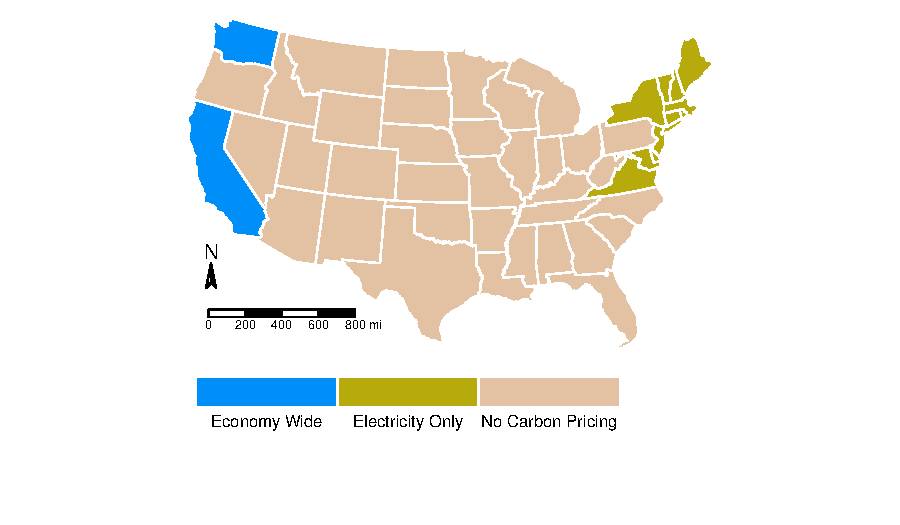
\includegraphics[width = \textwidth]{figures/chapter3_figures/cap_programs.pdf}
    \vspace*{-1.8cm}
    \fignote[1]{
        Figure displays statewide carbon pricing policies as of January 1, 2023 for the contiguous 48 states. Economy-wide cap-and-trade programs price emission from electricity, as well as other sectors, like industrial processes and transportation fuel distributors. Electricity-only cap-and-trade programs only pricing emissions from the electric power industry. Together, there are thritheen states with carbon tax or cap-and-trade programs at the state level in the US. The remaining 37 states do not have carbon pricing programs. Records from \cite{c2es_map}.
    }
\end{figure}

However, as Figure \ref{cap_states} shows, most of these states have programs that only cover emissions from electric power generation. These states on the East Coast all belong to the Regional Greenhouse Gas Initiative, an emissions trading scheme that applies only to fossil fuel powerplants in participating states. The cap-and-trade programs in California, Washington, and Quebec are all connected through the Western Climate Initiative, another market where participants can purchase emissions allowances. Unlike programs on the East coast, California and Washington's programs cover emissions outside of electricity, including some industrial emissions and transportation-related emissions. 

Outside of the US, carbon pricing is among the most popular decarbonization policies. The European Union has operated its own cap-and-trade program known as the Emissions Trading System (EU ETS) since 2005. The cap covers about 40\% of all greenhouse gas emissions in the EU primarily from electric power generation and other energy intensive industries \citep{eu_ets_overview}. Up until 2021, the EU ETS was the worlds largest carbon pricing system. In 2021, China began its own cap-and-trade program. Currently, China's cap-and-trade program covers only emissions from its electric power sector, but these emissions are substantial. The cap-and-trade system covers about 4.5 billion tonnes of CO$_2$ annually, twice the volume of emissions covered under the EU ETS. For comparison, the US totals around 5 billion tonnes of CO$_2$ annually. The Chinese government has stated that it plans to phase additional industries into the carbon pricing program as a part of its goal to peak emissions by 2030 and go carbon neutral by 2060 \citep{icap_report}. Globally, there are 70 carbon pricing initiatives (including national and subnational programs) which covered about 23\% of all CO$_2$e emissions in 2022 \citep{wbank}. 

Clearly carbon pricing is fairly popular among economists and policymakers around the world, but this does not reveal whether or not carbon pricing actually works. In general, it is difficult to assess the efficacy of carbon pricing programs ex-post. These programs usually are phased in slowly to ensure a smooth transition, a design that makes identifying the effect of these policies difficult because there are no sudden shocks that make for easy comparison of emissions pre- and post-implementation. Additionally, these programs are rarely if ever implemented in isolation. For instance, California's emissions trading program was first implemented alongside its clean energy portfolio standard. Again, this makes for a difficult comparison because we cannot easily identify what effects are attributable to the carbon pricing program and what effects are attributable to the other climate policies. Lastly, there is the trouble with the actual price of emissions. Even if researchers can overcome these other challenges and can identify the causal effect of a carbon pricing program on emissions, this will not have a clear implication for the emissions price. For instance, if the causal effect of a carbon pricing program on emissions is relatively small, then its not clear if the lack of efficacy is due to a flaw in the policy design or due to a price on emissions that is simply too low. Despite the challenges involved in evaluating the efficacy of carbon pricing programs, there is still plenty of room to glean insight on these programs. The remainder of this section overviews five key conclusions related to the function and success of carbon pricing. 

First, there is a desperate need for research that can offer an ex-post analysis of carbon pricing programs. Billions of dollars in allowances are already traded every year on emissions markets, yet credible ex-post analyses on the efficacy of these programs are scarce. This is no small task, and given the complexity of identification, this may only be possible if researchers collaborate with policymakers to implement policies in ways that will allow for strong ex-post analysis. \cite{green2021does} offers a timely meta-analysis of the existing literature on the effect of carbon pricing on emissions abatement. In her meta-analysis, Green finds just 37 papers from peer-reviewed journals, working papers series, and non-government entities that measure the effect of carbon pricing on emissions abatement. Most of these rely on dubious identification strategies, particularly matching on observables, which could potentially suffer substantially from omitted variable bias, and difference-in-differences, which has trouble with the many layered nature of treatments as well as dealing with the magnitude (price) of the treatment. Still, the meta-analysis suggests that often carbon pricing programs only result in emissions reductions between 0\% and 2\% annually, a finding that Green summarizes by stating ``[overall], the evidence indicates that carbon pricing has a limited impact on emissions.''

This apparent criticism motivates the second key takeaway: there is evidence that many of the jurisdictions that have already implemented carbon pricing programs rely extensively on other regulations to induce the majority of abatement. Given the lackluster performance of carbon pricing presented in \cite{green2021does}, this consideration is valuable for assessing the potential of carbon pricing in the future. Simply acknowledging that traditional regulations are currently creating more abatement does not represent a failure of carbon pricing, but instead reflects the preferences of policymakers. To see more impressive results from carbon pricing, the price of carbon must increase faster than the shadow price of other climate regulation.

\begin{figure}
	\centering
	\caption{Emissions Trading in Practice \label{c_pricing_prac}}
	\begin{tikzpicture}[scale=0.55]
		\draw[very thick, color3] (0, 3.5) -- (4, 3.5) -- (4, 4.5) -- (6, 4.5) -- (6, 5.5) -- (8, 5.5) -- (8, 6.5) -- (10, 6.5) -- (10, 10) node[above]{Cap$_2$};
		%\draw[very thick, color3] (0, 2.5) -- (8, 2.5) -- (8, 3.5) -- (10, 3.5) -- (10, 4.5) -- (12, 4.5); 
		\draw[very thick, gray] (6,0) node[below, black]{$E^*$} -- (6,10) node[above]{Cap$_1$};
		\draw[very thick, <->] (0,10) node[left]{$p$} -- (0,0) -- (13,0);	
		\draw[very thick, color2, domain=0:12] plot(\x, {8 - .5*\x}) node[right]{D = MB};
		\draw[very thick, color1, domain=0:12] plot(\x, {2 + .5*\x}) node[above right]{MSC};
		% \draw[very thick] (11, 0) node[below]{$E_\text{Current}$} -- (11, 10);
		\draw[very thick, dashed] (0,5) node[left, black]{$p^*$} -- (6,5);
		\node[below] at (6.5, -1) {CO$_2$e Emissions ($E$)};
	\end{tikzpicture}
	\fignote[1]{
		Figure displays the market for emissions under two different types of emissions ``caps.'' In this market, D = MB is the demand for emissions, MSC is the marginal social cost of emissions, $p^*$ is the equilibrium price of emissions, and $E^*$ is the equilibrium level of emissions. There are two potential caps in this market. Cap$_1$ illustrates the standard notion of a cap on emissions---a fixed quantity of emissions. Cap$_2$ illustrates a more realistic notion of the cap on emissions. With this ``cap,'' price increases can trigger the release of additional allowances, and price decreases can trigger cuts in the number of allowances available. 
	}
\end{figure}

To establish why policy analysts understand that in many jurisdictions complementary programs are responsible for the majority of emissions reductions, consider California's emissions trading program. California's emissions trading program differs in a few key ways from the traditional notion of a cap-and-trade program presented in Figure \ref{c_pricing}---as do most emissions trading programs. As it is typically imagined, the cap in a cap-and-trade program is a vertical supply curve for emissions allowances. This idea of an emissions cap appears as Cap$_1$ in Figure \ref{c_pricing_prac}. When the demand for emissions shifts, the price of allowances may change, but the quantity of emissions will not. In practice though emissions trading programs rarely have a set ``cap,'' hence why they are often called emissions trading programs rather than cap-and-trade programs. 

Instead, many emissions trading programs are structured as a hybrid between a carbon tax and a cap-and-trade program \citep{schmalensee2017lessons}. Cap$_2$ displays a more realistic supply curve for emissions allowance. Going left to right, there are three regions to this supply curve: (1) the absolute price floor, (2) the hybrid region, and (3) the absolute emissions cap. The absolute price floor is the lowest price the regulator will allow an allowance to sell at, like the starting price of an emissions allowance at auction. This portion of allowance supply curve behaves like a carbon tax in that polluters will pay a fixed price per tonne for their emissions. The absolute cap is the greatest number of allowances that the regulator will allow to go up for sale on the market. This portion of the allowance supply curve behaves like a traditional cap in that polluters cannot emit more than this set quantity. 
As \cite{schmalensee2017lessons} note, the hybrid region is composed of incremental emissions caps arranged like stairsteps or ``price collars.'' If the price of allowances increases enough above the absolute price floor, then this will trigger regulators to release additional emissions allowances. If the price of allowances increase above the minimum price at the previous step, this will again trigger regulators to release additional emissions allowances. This continues until the absolute emissions cap is reached, in which case higher allowance prices will not trigger the release of additional allowances.

The primary advantage of this design over of the standard cap-and-trade or carbon tax is reduced volatility. If the demand for allowances shifts, this design will result in a smaller change in price than a standard cap-and-trade program and a smaller change in emissions than a standard carbon tax. Providing this stability attracts investors and prevents firms from ``hoarding'' emissions allowances when they are cheap, in the hopes of using these permits later on when the cap becomes tighter. Now firms have some expectation that if there is a sudden spike in allowance prices, that regulators will release more permits to soften the blow. 

\begin{figure}
    \centering
    \caption{California Emissions Allowance Price \label{allowance_pr}}
    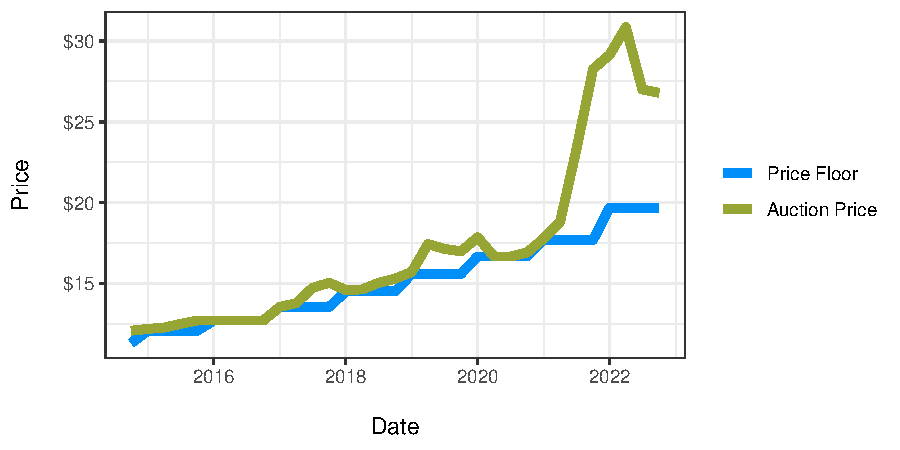
\includegraphics[width=\textwidth]{figures/chapter3_figures/allowance_prices.pdf}
    \fignote[1]{Figure displays the auction price and price floor for emissions allowances in California from Q4 2015 through Q4 2022. Each emissions allowance covers one tonne of CO$_2$e emissions. Data on emissions allowances come from the California Air Resources Board, \cite{carb_prices}.}
\end{figure}

For most emissions trading programs, the price of emissions allowances has remained near the absolute price floor for almost the entire history of the program. Figure \ref{allowance_pr} displays the price of California emissions allowances at auction alongside the price floor. Note first that regulators shift in the supply curve for emissions each year, a fact reflected in the annual increases in the absolute price floor. From most of the program's history, the auction price is just above the price floor. This took a turn in the first and second quarter of 2021, when prices spiked well above the price floor amidst the emergence of China's emissions market, a growing interest in holding emissions allowances as an asset, and anticipated tightening of the cap over the next decade \citep{storrow2022price}.\footnote{Allowance prices around the world substantially increased in 2021. This was particularly true in Europe, where the price per tonne of CO$_2$e briefly shot up to about \$100 per tonne before settling closer to \$80 per tonne \citep{manzagol2022global}. Under the Biden Administration, the social cost of carbon used in Federal studies is \$52 per tonne.} The price of carbon generally staying near the price floor is consistent with the suggestion that the existing cap is simply too high to create any substantial emissions reductions relative to other policies. 

There are of course alternative explanations for the proximity of allowance auction prices and the price floor. For instance, it could be that the price floor is just high relative to the shadow price of other regulations, in which case the price floor would be binding but the emissions trading program should be responsible for the majority emission reductions. If this were the case, then even high prices would not lead to abatement and we would have to conclude that carbon pricing is not effective in practice. In California though, policymakers have been clear that the reason allowance prices are near the absolute price floor is because emissions reductions are being led by other regulation. In an interview \citep{burtraw2022_rff}, Dallas Burtraw, the Chair of California's Independent Emissions Market Advisory Committee (IEMAC),\footnote{IEMAC is a group of researchers that advises the California Air Resources Board on how to manage its emissions trading program.} describes the policymaking process and the decisions that ensure this is the case:
\begin{quote}
	\singlespacing ``The primary way that emissions reductions have been achieved is \\through regulations and standards\ldots California has a process called the Scoping Plan process. It's a multiagency project, and they develop a blueprint for how the state's going to achieve its climate reduction goals. The first Scoping Plan identified over 80 percent of the emissions reductions that were needed to be achieved, associated with regulations, and only the remaining 20 percent (approximately) of emissions reductions were associated with the influence of the cap-and-trade program and the price of emissions allowances. The next Scoping Plans increase that share that was associated with the price effect of the cap-and-trade program up to the neighborhood of 40 percent.''
\end{quote}
This leads to the conclusion that if emission reductions from carbon pricing seem modest (as \cite{green2021does} suggests), it is because the price of emissions is just relatively low, not because the program is ineffective. Burtraw also indicates that California's cap-and-trade program is designed to take on a larger role in emissions reductions during the next phase of the state's climate strategy.

The third primary takeaway is the acknowledgement that current carbon pricing policies have room for improvement. For over a decade, policy scholars have understood two primary issues with carbon pricing: emissions leakage and carbon offsets \citep{cullenward2014carbon}. The next section considers emissions leakage in greater detail, but as a preview, emissions leakage may mean that carbon pricing just moves emissions into jurisdictions that do not have such stringent climate policy. It is possible in some scenarios that there could be a substantial volume of emissions that ``leak'' into other jurisdictions. It is also possible that certain strategies to prevent leakage might undermine the efficacy of the carbon price, namely the practice of distributing free allowances to select industries. Although this is an issue with carbon pricing, it is an also issue that arises with command-and-control climate policy. This means that if the counterfactual in mind is an alternative policy, emissions leakage is not a valid critique of carbon pricing.

Carbon offsets on the other hand are an issue unique to emissions trading programs. The idea of a carbon offset is straightforward; to lower their net emissions, polluters can pay for emissions sequestration or emissions abatement elsewhere rather than abate their own emissions. For instance, abatement options in the aviation industry are limited primarily to fuel switching, which has difficulty eliminating a majority of CO$_2$e emissions even with substantial investment in alternative fuels \citep{dray2022cost}. Instead, airline operators could reduce their net emissions by planting trees or by paying others to abate their emissions (i.e., an emissions allowance that is not confined to the regulated jurisdiction). Provided they truly represent emissions reductions, carbon offsets provide a strategy to reduce net emissions in the face of emissions that are difficult to abate.

The issue with carbon offsets is that they often do not represent real emissions reductions. As an example, \cite{west2020overstated} study carbon offsets generated by Reduced Emissions for Deforestation and Forest Degradation (REDD$+$) zones in the Brazilian Amazon. Carbon offsets for this program---established by the United Nations Framework Convention on Climate Change---are generated by saving forest that would otherwise be destroyed and unable to sequester greenhouse gas emissions. The trouble is of course getting an accurate measurement of the emissions reductions that this reduced deforestation creates. If companies were already planning on not clearing this land, then there is not really any emissions reduction. \cite{west2020overstated} use synthetic controls to establish the relevant counterfactual and do not find any significant evidence that REDD$+$ programs have actually mitigated deforestation. The researchers results suggest that of the 5.4 million tonnes of carbon offset credits certified, only about 30,000 tonnes of credits (0.56\%) are legitimate. 

Carbon offsets are widely understood by even non-researchers to be less effective than they appear, but not entirely ineffective \citep[see, for example,][]{astor2022airline}. As a result, emissions trading programs that accept carbon offsets are likely less effective than they appear as well. Still, there are legitimate efforts both to (1) make carbon offsets more credible, and (2) limit the use of carbon offsets in emissions trading. To the first point, California has attempted to improve the credibility of carbon offsets by limiting carbon offset credits to a list of projects that the state can verify \citep{carb_offsets}. To the second point, California limits the use of carbon offsets to 4\% of an entity's emissions obligation \citep{carb_offsets_about}. Carbon offsets are still a weak point for emissions trading programs, but a weak point that is increasing small in scope. 

Fourth, there is little reason to believe that carbon pricing is not effective. The previous takeaways have made clear that if carbon pricing programs appear ineffective relative to other emissions reduction programs, this is likely because the regulators have largely used carbon pricing in only a complementary role. Additionally, while carbon pricing programs are not perfect, the most significant issues are still small in scope. As a result, there is just not substantial, credible evidence that carbon pricing will not be effective at reducing emissions as regulators begin to prioritize these programs in the decarbonization planning. Other emissions trading programs for criteria air pollutants in the US have been highly successful \citep{schmalensee2017lessons}. Importantly, compliance rates for carbon pricing programs are extremely high; year after year, 100\% of businesses meet all their emissions obligations in California \citep{carb_comp_2018, carb_comp_2021}. Assuming the high rates of compliance continue, raising the carbon tax or reducing the cap must imply the corresponding level of emissions abatement. Carbon pricing can successfully reduce greenhouse gas emissions.

Of course the primary argument for the use of carbon pricing is not that it can reduce greenhouse gas emissions. After all, there are a variety of other policies that can also achieve emissions reductions. The primary argument for the use of carbon pricing is that it is cost-effective, a point that leads to the fifth and final takeaway on carbon pricing: in some contexts, there is also little reason to believe that carbon pricing is substantially more cost-effective than some command-and-control policies. \cite{borenstein2022carbon} provide good reason to believe that for the electric power industry, clean energy standards may come with a price tag comparable to a carbon tax. The explanation behind this is that there is a strong positive correlation between the social costs and private costs for ``dirty'' generation. A clean energy standard (CES) is a command-and-control policy that sets a minimum proportion of electricity in the state that must come from sources designated as ``clean''. Equivalently, a CES sets a maximum proportion of electricity that can come from ``dirty'' sources. Because a CES does not differentiate between generation within the ``dirty'' group, standard theory would predict that a CES will be inefficient---a coal plant might outlive a natural gas plant despite being far dirtier. However, within those power plants designated as ``dirty'' those are dirtier also tend to have higher marginal costs. This translates into an allocation of generation under a CES that is similar to the allocation of generation under a carbon price. Clean energy subsidies---which are usually thought to be even more inefficient, as they make electricity cheaper and thereby increase the quantity demanded of an emissions intensive good---may be efficient as well. Here the key is that retail electricity prices are already well above the socially optimal price, meaning that command-and-control subsidies may reduce emissions while moving prices in a socially optimal direction. 

The upshot of this is whether or not this result from the electric power industry generalizes to other industries as well. This question is more difficult because less is known about the private costs these firms face. Intuition suggests that this does not hold as well in other industries. Retail electricity prices well-above the socially optimal prices is a result of the unique pricing structure of electricity and there is little reason to believe this would be true of other emissions intensive industries like cement production. There is likely a correlation between social costs and private costs in other industries that stems from energy efficiency, but this correlation is also likely to be looser as these other industries will be less energy intensive than electric power generation. Overall, context is important when considering the cost savings that a carbon price offers over command-and-control regulations. 

% Chapter 2 describes arguments against carbon pricing that critique the efficacy of these programs. This discussion comes to four primary conclusions. First, there is a need for additional research that measures the ex-post effect of carbon pricing on emissions reductions. Second, many jurisdictions with carbon pricing programs have chosen to rely on other regulations to attain emissions targets. That is, the implicit price on emissions from other regulations is often higher than the market price of emissions, which can make the effect of emissions pricing appear weak relative to other regulations. Third, in situations where policymakers rely primarily on carbon pricing more so than other regulations, carbon pricing does appear to be the more cost-effective policy. This difference appears to be small though, especially in the electricity market where the strong correlation between the merit order of generation and emissions intensity mean that clean energy standards perform only negligibly worse carbon pricing. Fourth, there are likely tangible improvements to emissions trading programs that can be made, such as reforming or eliminating the use of emissions offsets. 



\subsection{Unilateral Climate Policy \& Leakage}

% \begin{quote}
% 	``You know these pest control companies. They call themselves exterminators, but they can't really do it. The best they can do is get the bugs to go to somebody else's house. They just relocate them, you know what I mean? They're bug realtors is what they are."\\ \\[-1.8ex]
% 	--- Jerry Seinfeld on the follies of incomplete regulation (Seinfeld, Season 6, Episode 19, ``The Doodle")
% \end{quote}

The previous section looked at the ability of carbon pricing to reduce greenhouse gas emissions within a closed economy. Although this is the standard presentation of carbon pricing, in actuality, carbon pricing occurs for open economies. This distinction creates potentially difficulties for many policies aimed at curbing emissions, including carbon pricing. 

When an individual jurisdiction takes up a carbon pricing program, this is known as \emph{unilateral} carbon pricing, meaning that this jurisdiction adopts the policy without coordinated carbon pricing schemes across all or most all other jurisdictions in its same trade network. This is the current state of carbon pricing programs. Recall that 23\% of all CO$_2$e emissions face a carbon price, meaning that the majority of emissions do not face a carbon price \citep{wbank}. Unilateral carbon pricing is an example of an incomplete regulation: a situation where not all relevant actors in the market face regulation. In the case of greenhouse gas emissions, everyone is a relevant actor, meaning that without a global carbon pricing scheme, any unilateral carbon pricing scheme will always be incomplete. For example, even if Country A has a price on its carbon, it will not be able to put a price on the emissions from Country B, even though Country B's emissions are just as damaging to Country A as its own emissions. That is not to say that unilateral carbon pricing schemes are not worth it, but to acknowledge that the policy misses some emissions. 

The purpose of this section is to explore the impacts of incomplete climate policy on the efficacy of this policy. Most of the examples focus on carbon pricing, but many of the discussion generalizes to other climate policies that create asymmetric regulation within markets. This begins with a discussion of how climate policy affects the geographic distribution of economic activity, and then moves on to consider both the implications of this redistribution on net emissions and the strategies available to address the issue.

A frequent claim of those opposing aggressive climate policy is that it will make the domestic economy ``less competitive" than foreign economies. That is, some claim that foreign firms will gain a greater global market share as a result of higher domestic regulatory costs. Understandably, the effect of climate and environmental policy on domestic economic activity is of considerable interest to not just economists, but policymakers and the general public.

Central to the debate among researchers on the topic are two competing perspectives: the pollution haven hypothesis and the Porter Hypothesis \citep{dechezlepretre2020impacts}. The pollution haven hypothesis holds that increasing domestic environmental policy stringency will make domestic firms relatively less competitive than foreign firms, shifting economic activity towards foreign economies. This claim is familiar; if the US implemented a nationwide carbon tax, then production prices in the US would rise relative to foreign production prices, leading consumers both in the US and abroad to buy fewer US goods. The Porter hypothesis, popularized in \cite{porter1995toward}, holds instead that increasing domestic environmental policy stringency will make domestic firms relatively \emph{more} competitive than foreign firms, shifting economic activity towards the domestic economy. The argument is that increasingly stringent environmental regulation induces efficiency improvements and R\&D investment that will result in lower domestic production costs, and ultimately a shift in economic activity towards the domestic economy. For instance, if a climate policy switches electricity generation from fossil fuels to renewables, this could lower the retail price of electricity and lower the costs of domestic producers. 

Contemporary empirical evidence on the pollution haven and Porter hypotheses leads to a few key conclusions: (1) environmental regulation does not have an economically significant effect on aggregate trade flows, and (2) environmental regulation can have an economically significant effect on the trade flows of specific industries that is consistent with the pollution haven hypothesis. A common technique for assessing differences in climate policies is considering differences in energy prices \citep[see, for example,][]{fowlie2022mitigating}. The idea is that carbon prices function in the short run by raising the price of energy that a firm's technology relies on. Using differences in energy prices as a proxy, \cite{sato2015asymmetric} show that a 10\% increase in the energy price gap between trading countries only increases bilateral manufacturing trades by 0.2\%. Further these same energy price differences only explain 0.01\% of the variation in trade flows. \cite{aldy2015competitiveness} find a null result in a similar study looking at energy price differences between US states---the effect of energy price differences on total manufacturing imports between states was statistically insignificant, even with their over thirty years of panel data. However, they do find pronounced effects in certain, energy intensive sectors including steel, industrial chemicals, and cement. Similarly, in their survey of the literature, \cite{dechezlepretre2020impacts} come to the conclusion that there is likely a pollution haven effect, but that it is confined to a select number of industries.


The existence of a pollution haven effect is interesting in its own right, but the effect on the relative competitiveness of domestic and foreign firms does not immediately speak to the efficacy of climate policy. Taken a step further though, it is clear that if climate policy shifts economic activity towards the foreign, under-regulated jurisdictions, this will also imply that the greenhouse gas emissions created by this economic activity shift into foreign jurisdictions as well. Unfortunately, even if the transfer of economic activity is small overall, the transfer of emissions can be quite large.

This is a part of a broader process known as \emph{emissions leakage} that occurs when the implementation of a stringent regulation on greenhouse gas emissions in one place leads to increased greenhouse gas emissions in another place with looser regulations. Assuming the goal of climate policy is to mitigate climate damages by reducing global emissions, rather than just hitting a domestic emissions target, then emissions leakage could seriously undermine the efficacy of climate policy. 

% Emissions leakage is closely related to the pollution haven hypothesis, but differs in a few ways. First, emissions leakage refers exclusively to GHG emissions, not pollution in general. This distinction is important as most GHG emissions have a negligible effect on the areas downwind from their source of emissions, but ambient air pollutants do not. Thus, the consequences of increased GHGs from emissions leakage is global rather than local. Second, the pollution haven hypothesis is much more concerned with international trade flows and the changing composition of economies, whereas emissions leakage is concerned more with changing the distribution of emissions. That is, the pollution haven hypothesis focuses on the implications of displaced economic activity, and emissions leakage focuses on the implications of displaced emissions.

\begin{figure}[!htbp]
\caption{Competitive Emissions Leakage \label{leakage_ex}}
\centering
\singlespacing
\footnotesize
\begin{tikzpicture}[scale = 0.5]
	\draw[very thick, <->] (0, 11) node[left]{$p$} -- (0, 0) -- (11, 0) node[below, text width = 2cm]{Domestic Quantity};
	\draw[very thick, <->] (15, 11) node[left]{$p$} -- (15,0) -- (26, 0) node[below, text width = 2cm]{Imported Quantity};
	\fill[yellow!80!, opacity = 0.6] (3.5, 3.75) -- (3.5, 1.75) -- (4.5, 2.25) -- (4.5, 4.25) -- cycle;
	\fill[yellow!80!, opacity = 0.6] (4.5, 2.25) -- (5.5, 2.75) -- (5.5, 4.75) -- (4.5, 4.25) -- cycle;
	\fill[orange!80!, opacity = 0.6] (16.75, 4.75) -- (16.75, 2.75) -- (17.75, 3.75) -- (17.75, 5.75) -- cycle;
	%\fill[orange!80!, opacity = 0.6] (16.25, 4.25) -- (16.25, 2.25) -- (16.75, 2.75) -- (16.75, 4.75) -- cycle;
	\fill[red!80!, opacity = 0.6] (21.25, 9.25) -- (21.25, 7.25) -- (22.25, 8.25) -- (22.25, 10.25) -- cycle;
	%\fill[red!80!, opacity = 0.6] (20.75, 8.75) -- (20.75, 6.75) -- (21.25, 7.25) -- (21.25, 9.25) -- cycle;
	\draw[very thick, color1] (0,0) -- (10, 5) node[right]{MC$_d$};
	\draw[very thick, color3] (0,2) -- (10, 7) node[right]{MC$_d$ $+$ Tax};
	\draw[very thick, gray] (0, 10) -- (10,0) node[pos=.2, above right,text width = 1.5cm]{Domestic Demand}; 
	\draw[very thick, color2] (0,5.5) -- (9, 1) -- (10, 0) node[pos=.8, above right, text width = 1.5cm]{Residual Demand};
	%\draw[very thick, color2] (0, 6.5) -- (7,3) -- (10, 0);
	\draw[very thick, gray] (15, 10) -- (25, 0) node[pos=.8, above right,text width = 1.5cm]{Domestic Demand}; 
	\draw[very thick, color1] (15, 1) -- (24, 10) node[right, text width = 1.5cm]{MC$_f$};
	\draw[dashed, thick] (5.5, 4.75) -- (5.5, 0) node[below, yshift = -3pt]{$q_d$};
	\draw[dashed, thick] (3.5, 3.75) -- (3.5, 0) node[below]{$q_d'$};
	%\draw[dashed, thick] (4.5, 4.25) -- (4.5, 0) node[below]{$q_d''$};
	\draw[dashed, thick] (0, 3.75) node[left]{$p'$} -- (21.25, 3.75);
	\draw[dashed, thick] (0, 2.75) node[left]{$p$} -- (22.25, 2.75);
	%\draw[dashed, thick] (0,4.25) node[left]{$p''$} -- (20.75, 4.25);
	\draw[dashed, thick] (16.75,4.75) -- (16.75, 0) node[below, yshift = -3pt]{$q_f$};
	\draw[dashed, thick] (17.75, 5.75) -- (17.75, 0) node[below]{$q_f'$};
	%\draw[dashed, thick] (16.25, 4.25) -- (16.25, 0) node[below]{$q_f''$};
	\draw[dashed, thick] (22.25, 10.25) -- (22.25, 0) node[below, yshift = -3pt]{$q$};
	\draw[dashed, thick] (21.25, 9.25) -- (21.25, 0) node[below]{$q'$};
	%\draw[dashed, thick] (20.75, 8.75) -- (20.75, 0) node[below]{$q''$};
	\draw[dotted] (15, 3) -- (23, 11) node[right]{MC$_f$ $+$ Tax};
	\draw[thick, <-] (5, 4) -- (8, 8) node[above, text width = 2cm, align=center]{Domestic Abatement};
	\draw[thick, <-] (17.4, 4.5) -- (18.2, 8) node[above, text width = 2cm, align=center]{Emissions Leakage}; 
		\draw[thick, <-] (21.7, 8.2) -- (23, 6) node[below right, text width = 1.6cm, align=center]{Net Abatement};
		\node at (5.5, 12) {Domestic Market};
		\node at (20.5, 12) {Import Market}; 
\end{tikzpicture}
\vspace*{1em}
\fignote[1]{
	Figure adapted from Figure 2 in \cite{fowlie2016measuring} depicts the domestic market and import market for an EITE good. Residual demand in the domestic market is calculated as the difference between the quantity demanded and the quantity supplied in the import market. Subscripts of $d$ denote a domestic quantity ($q$) or marginal cost (MC), and $f$ denote a foreign quantity or marginal cost. Quantities and prices ($p$) with an $'$ are after the carbon tax has been applied, and quantities and prices without an $'$ are before the carbon tax has been applied. The yellow shaded region represents the value of domestic emissions reductions, the orange shaded region represents the cost of increases in foreign emissions (i.e., emissions leakage), and the red shaded region represents the value of the net emissions abatement.
}
\end{figure}

Figure \ref{leakage_ex} displays how competitive effects can drive emissions leakage in the market for an emissions-intensive good. In the left panel of Figure \ref{leakage_ex} is the domestic market for an arbitrary emissions-intensive good. In the right panel of Figure \ref{leakage_ex} is the import market for the same good. Domestic producers do not face the full domestic demand curve, as foreign producers will also be willing to supply the domestic market. Instead, domestic producers face the residual demand curve---the difference between the domestic quantity demanded and the import supply at each price. Domestic firms will produce where their marginal cost curve MC$_d$ intersects residual demand. This price then caries into the import market, and foreign firms will produce where the domestic market price intersects their marginal cost curve MC$_f$. Absent any carbon pricing scheme, domestic firms produce $q_d$, foreign firms import $q_f$, and the total market quantity is $q$. 

Now suppose that domestic policymakers implement a carbon pricing scheme. For ease, assume that this takes the form of a per tonne emissions tax and that marginal emissions and marginal damages from emissions are both constant. The carbon pricing scheme is unilateral, meaning that it applies to all domestic producers, but not any foreign producers. The constant marginal emissions rate and per unit carbon tax imply that domestic firms pay a constant per unit tax on their output, creating a parallel shift up in from MC$_d$ to MC$_d$ $+$ Tax. Again, firms produce where the marginal cost they face equals residual demand. This causes the domestic price of the good to rise to $p'$ and the domestic production of the good to fall to $q_d'$. The yellow region of left panel in figure \ref{leakage_ex} represents a monetary measure of domestic abatement. If the tax on emissions is set equal to the social cost of a tonne of emissions, then this area is the monetary value of all domestic emissions abatement, $\text{Tax} \times E \times (q_d' - q_d)$, where $E$ is the emissions intensity of the good measured in tonnes CO$_2$e per unit. Like we should expect, the carbon pricing scheme induces domestic reductions in emissions.

Unfortunately, this is not the case in the import market. Unlike firms in the domestic market, foreign firms do not face this same emissions price. Higher prices in the domestic market without the counteracting increase in costs induce foreign firms to expand their production from $q_f$ to $q_f'$. Analogous to the yellow area, the orange area in the right panel of figure \ref{leakage_ex} represents the social cost of the additional emissions in the import market, $\text{Tax} \times E \times (q_f' - q_f)$. This is emissions leakage: an increase foreign emissions as a result of unilateral carbon pricing. Still, unilateral carbon pricing manages to reduce total emissions despite the leakage. Total quantity in the domestic market falls from $q$ to $q'$, with the area of the red region representing the social value of the net abatement, $\text{Tax} \times E \times (q' - q)$. This example demonstrates that with a climate policy, like a carbon tax, the global emissions reductions may be more modest than what domestic emissions might portray. 

There is a certain class of goods that are particularly susceptible to emissions leakage known as \emph{emissions-intensive and trade-exposed} (EITE) goods. A good is emissions intensive if its production creates  a high volume of emissions per unit (tonnes of CO$_2$e/\text{Chained} \$). The trade exposure of a good is the ratio of the volume traded domestically (value of imports $+$ value of exports) to the total volume of good that passes through the domestic economy (value of domestic production $+$ value of imports). \cite{fowlie2022mitigating} and \cite{fowlie2016measuring} show that it is not enough to be only emissions intensive or only trade exposed to have a high risk of leakage. Both conditions are necessary to have a substantial risk of emissions leakage. EITE goods include cement, steel, and many industrial chemicals.

The bad news of emissions leakage does not end there. There are many ways that emissions leakage can occur. Using the language of \cite{cosbey2020developing}, we have so far discussed the competitiveness channel, where emissions increase outside of the regulated jurisdiction as unregulated producers become more competitive. Another important form of leakage occurs through the energy market channel. If the US implemented a stringent tax on greenhouse gases from cars, the domestic demand for gasoline will fall dramatically as US commuters opt for modes of transportation other than gas-fueled vehicles (e.g., electric vehicles, bikes, public transit). The US is large enough though that this will cause prices to fall in global energy markets, and when petroleum-based fuels become cheaper, more firms will begin using petroleum-based fuels and creating more emissions elsewhere. These general equilibrium effects that move in and around global energy markets are difficult to address without globally coordinated efforts to ditch fossil fuels. These two channels are thought to be the primary drivers of leakage \citep{branger2014climate}

There are also a few ways where we might see negative emissions leakage. That is, situations where ambitious steps towards abatement in one location spillover into abatement somewhere else.\footnote{Just as emissions leakage pulls intuition from the pollution haven hypothesis, negative emissions leakage pulls intuition from the Porter hypothesis.} The income channel provides opportunity for negative leakage. If a carbon tax makes people poorer in less-regulated jurisdictions, then this could decrease foreign consumption and production of emissions intensive goods and lower emissions. Of course, this is not a favorable way to reduce emissions. The income channel could operate in the opposite direction as well, raising emissions in places where incomes increase as a result of the incomplete regulation. The more likely form of negative leakage occurs through the technology channel. Carbon pricing schemes reduce emissions not just by internalizing the externality, but by providing incentives for the creation of new, cleaner technologies. Producers facing emissions pricing certainly have an incentive to adopt cleaner technologies, but producers outside of the regulated region do not have this same carrot and stick. If these new technologies happen to be more cost-effective than existing technologies, then it is possible that producers would adopt these cleaner technologies and reduce emissions this way. The prospect of negative emissions leakage is overly optimistic as a whole, and empirical evidence to date suggests that negative leakage is negligible compared to the other channels of leakage \citep{winchester2013numerical}.

\cite{fowlie2018challenges} summarize briefly the two primary difficulties researchers face when attempting to measure emissions leakage. First, researchers need data on the emissions intensity of foreign producers. The current standard practice is to use sectoral averages of emissions intensities, which provide a good benchmark, but ultimately may differ from the true emissions intensity due to wide variation in emissions intensities within an industry and foreign emissions intensities that are endogenous to the policy itself. Second, researchers need to measure the elasticity of foreign supply with respect to the domestic carbon price. Like emissions intensity measures, a highly aggregated elasticity can contribute to uncertainty in the estimated emissions leakage. The primary concern though is uncertainty in this elasticity itself, which can lead to substantial changes in the estimated magnitude of emissions leakage. 

Nevertheless, there are numerous empirical reviews in the economics literature that attempt to measure the magnitude of emissions leakage that result from domestic climate policy. Economists typically use computable general equilibrium (CGE) models to model changes in international trade flows that result from climate policy, and then apply sectoral averages of emissions intensities. In a meta-analysis of these CGE studies, \cite{carbone2017impacts} analyze the results of 291 different simulations from 54 different papers. They find that in the majority of policy simulations, EITE industries experience emissions leakage rates between 20 and 30 percent. That is, for every 10 tonnes CO$_2$e of domestic abatement in these industries, foreign emissions increase between 2 and 3 tonnes CO$_2$e. 

Clearly emissions leakage does not render unilateral climate policy in EITE sectors useless, but it does diminish the its efficacy. Recall that leakage occurs due to regulatory asymmetries. To mitigate the risk of emissions leakage, jurisdictions might attempt to even these asymmetries by adjusting the prices of imports and exports so all goods face a similar set of regulations. These policies are called border carbon adjustments (BCAs), and they come in two major varieties: import charges (or taxes) and export (or output) rebates. Import charges attempt to complete the regulation of domestic markets by subjecting foreign imports to carbon prices similar to the carbon prices domestic producers pay. In the US, import charges are the more relevant of the two major varieties of BCAs, largely because the US imports more EITE goods than it exports. 

Figure \ref{import_charge} displays how an emissions charge on imports can reduce leakage. As in Figure \ref{leakage_ex}, suppose that domestic firms pay a constant tax for each tonne CO$_2$e. For simplicity, assume that all producers, domestic and foreign, have a constant, identical emissions intensity. With the unilateral emissions tax and without an import charge, there is substantial domestic abatement---represented by the orange and yellow regions in the domestic market---and there is substantial leakage---represented by the red region in the import market. The total emissions reductions are represented by the violet region in the import market. 

Consider now when policymakers impose an import charge analogous to the domestic emissions tax. Now foreign producers face MC$_f$ $+$ Tax, a parallel shift of their previous marginal cost curve. With the marginal cost curve shifting back in the import market, the difference between the domestic quantity demanded and the quantity of imports supplied increases at every price level. As a result, residual demand in the domestic market shifts up. Setting this new residual demand curve RD$''$ equal to the marginal cost MC$_d$ $+$ Tax, increases the domestic quantity from $q_d'$ to $q_d''$. This means that the value of domestic abatement decreases from the sum of areas of the orange and yellow regions in domestic market to just the area of the yellow region. Although there is modest increase in domestic emissions due to the import charge, there is larger reduction in foreign emissions. The import charge moves foreign production from $q_f'$ to $q_f''$. Previous to the imposition of the import charge, the unilateral emissions tax increased the costs of foreign emissions by the area of the red region in the import market. With the imposition of the import charge though, we see that foreign emissions are actually less than they were in the baseline (no domestic emissions tax and no import charge). The social value of this foreign abatement is give by the area of the region in blue. The total quantity of the good in the domestic market decreases from $q_d'$ to $q_d''$. The additional social value of emissions abatement due to the import charge is given by the area of the green region in the import market.

\begin{figure}
\caption{Leakage with an Import Charge \label{import_charge}}
\centering
\singlespacing
\footnotesize
\begin{tikzpicture}[scale = 0.5]
	\draw[very thick, <->] (0, 11) node[left]{$p$} -- (0, 0) -- (11, 0) node[below, text width = 2cm]{Domestic Quantity};
	\draw[very thick, <->] (15, 11) node[left]{$p$} -- (15,0) -- (26, 0) node[below, text width = 2cm]{Imported Quantity};

	\fill[color2!80!, opacity = 0.6] (3.5, 3.75) -- (3.5, 1.75) -- (4.5, 2.25) -- (4.5, 4.25) -- cycle;
	\fill[yellow!80!, opacity = 0.6] (4.5, 2.25) -- (5.5, 2.75) -- (5.5, 4.75) -- (4.5, 4.25) -- cycle;
	\fill[orange!80!, opacity = 0.6] (16.75, 4.75) -- (16.75, 2.75) -- (17.75, 3.75) -- (17.75, 5.75) -- cycle;
	\fill[color1!80!, opacity = 0.6] (16.25, 4.25) -- (16.25, 2.25) -- (16.75, 2.75) -- (16.75, 4.75) -- cycle;
	\fill[red!80!, opacity = 0.6] (21.25, 9.25) -- (21.25, 7.25) -- (22.25, 8.25) -- (22.25, 10.25) -- cycle;
	\fill[violet!80!, opacity = 0.6] (20.75, 8.75) -- (20.75, 6.75) -- (21.25, 7.25) -- (21.25, 9.25) -- cycle;

	\draw[very thick, color1] (0,0) -- (10, 5) node[right]{MC$_d$};
	\draw[very thick, color3] (0,2) -- (10, 7) node[right]{MC$_d$ $+$ Tax};
	\draw[very thick, gray] (0, 10) -- (10,0) node[pos=.2, above right,text width = 1.5cm]{Domestic Demand}; 
	\draw[very thick, gray] (0,5.5) -- (9, 1) -- (10, 0) node[pos=.5, left, xshift = -2pt]{RD};
	\draw[very thick, color2] (0, 6.5) -- (7,3) -- (10, 0) node[pos=.8, above right, text width = 1.5cm]{RD''};
	\draw[very thick, gray] (15, 10) -- (25, 0) node[pos=.8, above right,text width = 1.5cm]{Domestic Demand}; 
	\draw[very thick, color1] (15, 1) -- (24, 10) node[right, text width = 1.5cm]{MC$_f$};
	\draw[dashed, thick] (5.5, 4.75) -- (5.5, 0) node[below]{$q_d$};
	\draw[dashed, thick] (3.5, 3.75) -- (3.5, 0) node[below]{$q_d'$};
	\draw[dashed, thick] (4.5, 4.25) -- (4.5, 0) node[below]{$q_d''$};
	\draw[dashed, thick] (0, 3.75) node[left]{$p'$} -- (21.25, 3.75);
	\draw[dashed, thick] (0, 2.75) node[left]{$p$} -- (22.25, 2.75);
	\draw[dashed, thick] (0,4.25) node[left]{$p''$} -- (20.75, 4.25);
	\draw[dashed, thick] (16.75,4.75) -- (16.75, 0) node[below, yshift = -3pt, xshift = 2pt]{$q_f$};
	\draw[dashed, thick] (17.75, 5.75) -- (17.75, 0) node[below]{$q_f'$};
	\draw[dashed, thick] (16.25, 4.25) -- (16.25, 0) node[below]{$q_f''$};
	\draw[dashed, thick] (22.25, 10.25) -- (22.25, 0) node[below]{$q$};
	\draw[dashed, thick] (21.25, 9.25) -- (21.25, 0) node[below]{$q'$};
	\draw[dashed, thick] (20.75, 8.75) -- (20.75, 0) node[below]{$q''$};
	\draw[color3, very thick] (15, 3) -- (23, 11) node[right]{MC$_f$ $+$ Tax};

	\draw[very thick] (3.5, 3.75) -- (3.5, 1.75) -- (4.5, 2.25) -- (4.5, 4.25) -- cycle;
	\draw[very thick] (16.25, 4.25) -- (16.25, 2.25) -- (17.75, 3.75) -- (17.75, 5.75) -- cycle;
	\draw[very thick] (20.75, 8.75) -- (20.75, 6.75) -- (21.25, 7.25) -- (21.25, 9.25) -- cycle;
	\draw[thick, <-] (3.8, 3.2) -- (8, 8) node[above, text width = 2cm, align=center]{$\Delta$Domestic Emissions};
	\draw[thick, <-] (16.8, 4.4) -- (18, 8) node[above, text width = 2cm, align=center]{$\Delta$Emissions Leakage}; 
	\draw[thick, <-] (21, 7.7) -- (23, 6) node[below right, text width = 1.6cm, align=center]{$\Delta$Net Abatement};
	\node at (5.5, 12) {Domestic Market};
		\node at (20.5, 12) {Import Market}; 
\end{tikzpicture}
\vspace*{1em}
\fignote[1]{
	Residual demand in the domestic market is calculated as the difference between the quantity demanded and the quantity supplied in the import market. Subscripts of $d$ denote a domestic quantity ($q$) or marginal cost (MC), and $f$ denote a foreign quantity or marginal cost. Quantities and prices ($p$) with an $'$ are after the carbon tax has been applied, quantities and prices without an $'$ are before the carbon tax has been applied, and quantities with an $''$ are after the import charge. Different from Figure \ref{leakage_ex}, here importers actually face an identical tax, shifting the marginal costs in the import market to the left. Together, the green and yellow shaded region represent the value of domestic emissions reductions with no import charge, the orange shaded region represents the cost of increases in foreign emissions (i.e., emissions leakage) with no import charge, and the red shaded region represents the value of the net emissions abatement with no import charge. The green shaded region represents the cost ofn increases in domestic emissions, the blue and orange region together represent the value of emissions reductions in foreign emissions, and the violet region represents the value of the increase in net abatement, all associated with the import charge.
}
\end{figure}

% Before we determine how to assess the emissions of imported goods, it is useful to know how we assess the emissions of domestically produced goods. The GHG Protocol, the internationally recognized leader in GHG emissions accounting standards, sets out three emissions scopes. Scope 1 looks at just an organization's direct emissions, like the GHGs that the organization emits on site. Scope 2 includes all these direct emissions from Scope 1, but also includes indirect emissions associated with energy inputs. For instance, a database center might have relatively low Scope 1 emissions, but if all electric power needed for the database center comes from a coal-fueled plant, Scope 2 emissions would be high. Scope 3 takes this a step further to look at the lifecycle emissions associated with an organization. This includes all the emissions captured by Scope 2, and includes emissions embodied in non-energy inputs and downstream emissions from distribution, processing, use, and disposal of its output. Any domestic emissions pricing program first needs to determine what emissions it will use to assess emissions to firms. It is best practice to assess foreign emissions with the same scope as domestic emissions, and likely violates international trade law to assess emissions using a higher scope for foreign producers \citep{cosbey2020developing}.

% \begin{figure}
% 	\caption{Greenhouse Gas Emissions Scopes \citep{ghg_protocol_2011}\label{scopes}}
% 	\centering
% 	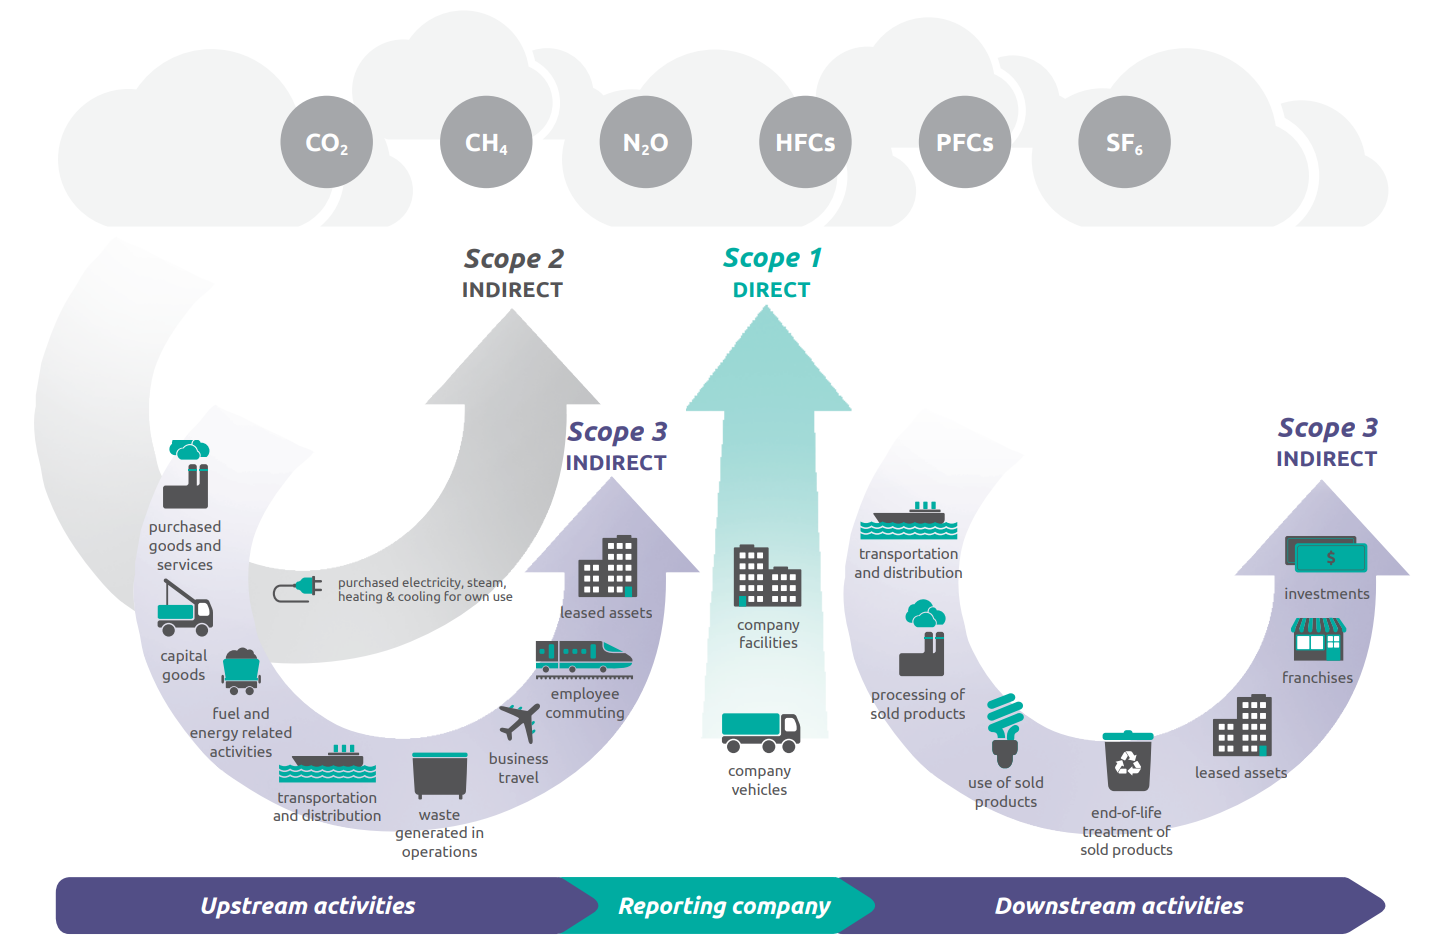
\includegraphics[width=0.8\textwidth]{figures/chapter2_figures/ghg_scope.png}
% \end{figure}

In their most complete form, border carbon adjustments cover all goods that cross the border, not just imports. Just like highly-regulated domestic production will likely have a cost disadvantage in the domestic market, highly-regulated exports will likely have a cost disadvantage in foreign markets. To prevent jurisdictions with ambitious climate policy from losing their exports requires some way to adjust the price of exports. This is the purpose of an export rebate, often just called an output rebate.

An output rebate pays back a flat rate to domestic producers for every unit they export. While carbon taxes on imports try to even the playing field between highly regulated and less regulated producers in domestic markets, output rebates try to even the playing field between highly regulated and less regulated producers on foreign markets. For instance, if US fertilizer manufacturers export much of their product, imposing a domestic carbon tax raises these manufacturers' costs relative to their competitors overseas. This cost differential may allow foreign fertilizer manufacturers to retake some of the (foreign) market share from US fertilizer manufacturers. This increased foreign production will lead to greater GHG emissions associated with the foreign fertilizer market, a problem that may be exacerbated if foreign manufacturers were already more emissions intensive than US manufacturers.

Output rebates lack some of the same intuitive appeal that an emissions tax on imports have. After all, why should regulators tax manufacturers only to pay them back? Why not just tax manufacturers the difference between the original emissions tax and the output rebate? The first reason is a matter of accounting. Output rebates only apply to exports, so reducing the tax on all goods would not differentiate between the goods that should and should not receive a subsidy to avoid leakage. The second reason is a matter of incentives. Output rebates are not refunds on emissions taxes, as the government pays these out for every unit of output rather than for every tonne of GHG emissions. In a world where goods had a fixed emissions intensity, this difference would not matter. Thankfully though, there are ways to reduce emissions without reducing output (e.g., switching to cleaner inputs or installing smokestack scrubbers). Thus, an output rebate will maintain the same abatement incentive on exports, while also allowing domestic producers to maintain their ability to compete in foreign markets. The low volume of US manufacturing exports relative to imports means that these are not typically the primary concern in anti-leakage policy.

To summarize, carbon pricing and many other climate policies suffer from their unrequited, unilateral nature. Asymmetric climate regulation provides competitive advantages to firms in less-regulated jurisdictions, a result with a strong backing in theory and evidence for a select number of industries. The two key characteristics of these industries are a high emissions intensity (high ratio of emissions to output) and a high trade exposure (highly traded). In these industries, climate policy can ``leak'' emissions to other jurisdictions, undermining domestic emissions abatement. To combat this, jurisdictions with stringent environmental policy relative to their trading partners can implement border carbon adjustments (BCAs) to reduce regulatory disparities in both domestic and foreign markets. These policies will be key in ensuring that packages of climate policy, including carbon pricing programs, can effectively reduce the global level of emissions.  


% \begin{figure}
% \caption{Leakage with an Emissions Tax on Imports}
% \centering
% \singlespacing
% \footnotesize
% \begin{tikzpicture}[scale = 0.5]
% 	\draw[very thick, <->] (0, 11) node[left]{$p$} -- (0, 0) -- (11, 0) node[below, text width = 2cm]{Domestic Quantity};
% 	\draw[very thick, <->] (15, 11) node[left]{$p$} -- (15,0) -- (26, 0) node[below, text width = 2cm]{Imported Quantity};
% 	\fill[orange!80!, opacity = 0.6] (3.5, 3.75) -- (3.5, 1.75) -- (4.5, 2.25) -- (4.5, 4.25) -- cycle;
% 	\fill[yellow!80!, opacity = 0.6] (4.5, 2.25) -- (5.5, 2.75) -- (5.5, 4.75) -- (4.5, 4.25) -- cycle;
% 	\fill[orange!80!, opacity = 0.6] (16.75, 4.75) -- (16.75, 2.75) -- (17.75, 3.75) -- (17.75, 5.75) -- cycle;
% 	\fill[yellow!80!, opacity = 0.6] (16.25, 4.25) -- (16.25, 2.25) -- (16.75, 2.75) -- (16.75, 4.75) -- cycle;
% 	\fill[orange!80!, opacity = 0.6] (21.25, 9.25) -- (21.25, 7.25) -- (22.25, 8.25) -- (22.25, 10.25) -- cycle;
% 	\fill[yellow!80!, opacity = 0.6] (20.75, 8.75) -- (20.75, 6.75) -- (21.25, 7.25) -- (21.25, 9.25) -- cycle;
% 	\draw[very thick, color1] (0,0) -- (10, 5) node[right]{MC$_d$};
% 	\draw[very thick, color3] (0,2) -- (10, 7) node[right]{MC$_d$ $+$ Tax};
% 	\draw[very thick, gray] (0, 10) -- (10,0) node[pos=.2, above right,text width = 1.5cm]{Domestic Demand}; 
% 	\draw[very thick, color2] (0,5.5) -- (9, 1) -- (10, 0) node[pos=.8, above right, text width = 1.5cm]{Residual Demand};
% 	\draw[very thick, color2] (0, 6.5) -- (7,3) -- (10, 0);
% 	\draw[very thick, gray] (15, 10) -- (25, 0) node[pos=.8, above right,text width = 1.5cm]{Domestic Demand}; 
% 	\draw[very thick, color1] (15, 1) -- (24, 10) node[right, text width = 1.5cm]{MC$_f$};
% 	\draw[dashed, thick] (5.5, 4.75) -- (5.5, 0) node[below]{$q_d$};
% 	\draw[dashed, thick] (3.5, 3.75) -- (3.5, 0) node[below]{$q_d'$};
% 	\draw[dashed, thick] (4.5, 4.25) -- (4.5, 0) node[below]{$q_d''$};
% 	\draw[dashed, thick] (0, 3.75) node[left]{$p'$} -- (21.25, 3.75);
% 	\draw[dashed, thick] (0, 2.75) node[left]{$p$} -- (22.25, 2.75);
% 	\draw[dashed, thick] (0,4.25) node[left]{$p''$} -- (20.75, 4.25);
% 	\draw[dashed, thick] (16.75,4.75) -- (16.75, 0) node[below, yshift = -3pt, xshift = 2pt]{$q_f$};
% 	\draw[dashed, thick] (17.75, 5.75) -- (17.75, 0) node[below]{$q_f'$};
% 	\draw[dashed, thick] (16.25, 4.25) -- (16.25, 0) node[below]{$q_f''$};
% 	\draw[dashed, thick] (22.25, 10.25) -- (22.25, 0) node[below]{$q$};
% 	\draw[dashed, thick] (21.25, 9.25) -- (21.25, 0) node[below]{$q'$};
% 	\draw[dashed, thick] (20.75, 8.75) -- (20.75, 0) node[below]{$q''$};
% 	\draw[color2, very thick] (15, 3) -- (23, 11) node[right]{MC$_f$ $+$ Tax};
% 	%\draw[thick, <-] (5, 4) -- (8, 8) node[above, text width = 2cm, align=center]{Domestic Abatement};
% 	%\draw[thick, <-] (16.7, 4.5) -- (18, 8) node[above, text width = 2cm, align=center]{Emissions Leakage}; 
% 	%\draw[thick, <-] (21.6, 8) -- (23, 6) node[below right, text width = 1.6cm, align=center]{Net Abatement};
% 	\node at (5.5, 12) {Domestic Market};
% 	\node at (20.5, 12) {Foreign Imports}; 
% \end{tikzpicture}
% \end{figure}

% %%%%%%%%%%%